\chapter{Theoretical foundations}
\label{chap:theoretical-foundations}

\section{Probability theory}
\label{sec:some-probability}

Our computations are based on fundamental probability theoretic considerations. We therefore introduce some important concepts, where we rely on established notation (i.e. we use $\p{}$ to denote probabilities, $\E{}$ for expected values, etc).

\subsection{Exponential distribution}
\label{sec:exponential-distribution}

The well-known exponential distribution is the central distribution we are dealing with in this text. All definitions and theorems within this subsection are along the lines of \cite{schickinger2001diskrete}.

\begin{definition}
  A continuous random variable is \emph{exponentially distributed} with parameter $\lambda$ if it has density 
  \begin{equation*}
    f(x) =
    \begin{cases}
      \lambda \cdot e^{-\lambda x} & \text{ if } x \geq 0 
      \\ 0 & \text{ otherwise}
    \end{cases}
    .
  \end{equation*}
\end{definition}

Note that the above definition also determines the distribution function $F$ of an exponentially distributed random variable as follows:

\begin{equation*}
  F(x) =
  \begin{cases}
    1-e^{\lambda x} & \text{ if } x \geq 0 \\
    0 & \text{ otherwise}
  \end{cases}
\end{equation*}

\begin{theorem}
  \label{thm:exponential-distribution-expectancy}
  Let $X$ be an exponentially distributed random variable. Then, the expectancy of $X$ is $\E{X} = \frac 1 \lambda$.
\end{theorem}

\begin{proof}
  We can compute the expectancy for $X$ as follows:
  \begin{eqnarray*}
    \E{X} 
    &=& \int_{-\infty}^\infty x\cdot f(x)\, dx = \\
    &=& \int_{0}^\infty x\cdot \lambda e^{-\lambda x}\, dx \\
    &=& \left[ - \frac{e^{-\lambda x}\cdot \left( \lambda x + 1 \right)}{\lambda} \right]_{0}^\infty \\
    &=& \frac{1}{\lambda}
  \end{eqnarray*}
\end{proof}

\begin{theorem}[Scalability]
  \label{thm:expoenential-distr-scalability}
  Let $X$ be an exponentially distributed random variable with parameter $\lambda$ and let $a\in \mathbb{R}^+$. Then, the random variable $aX$ is exponentially distributed with parameter $\frac{\lambda}{a}$.
\end{theorem}

\begin{proof}
  We compute the probability that the random variable $aX$ is less than $x$:
  \begin{equation*}
    \p{aX \leq x} 
    = \p{X \leq \frac{x}{a}}
    = 1 - e^{-\frac{\lambda}{a} \cdot x}
  \end{equation*}
  This result is equivalent to the density function of an exponentially distributed random variable with parameter $\frac{\lambda}{a}$.
\end{proof}

\begin{theorem}
  \label{thm:minimum-of-exponential-distribution-is-exponential}
  Let $X_1,\dots,X_n$ be exponentially-distributed random variables with respective parameters $\lambda_1,\dots,\lambda_n$. Then, the ranvom variable $Z:=\min_{i\in\left\{ 1,\dots,n \right\}} \left\{ X_i \right\}$ is exponentially distributed with parameter $\lambda=\lambda_1+\dots+\lambda_n$.
\end{theorem}

\begin{proof}
  We prove the claim by induction. 

  Suppose, we have two exponentially distributed random variables $X_1$ resp. $X_2$ with parameters $\lambda_1$ resp. $\lambda_2$. We then can compute
  \begin{align*}
    \p{min\left\{ X_1,X_2 \right\} \geq x} & = \p{X_1 \geq x \wedge X_2 \geq x} = \\ 
    & = \p{X_1 \geq x}\cdot\p{X_2 \geq x} = \\
    & = e^{-\lambda_1 x} \cdot e^{-\lambda_2 x} = \\
    & = e^{-\lambda_1 x - \lambda_2 x} = \\
    & = e^{-\left( \lambda_1+\lambda_2 \right) \cdot x},
  \end{align*}
  from which we can conclude that $\min\left\{ X_1,X_2 \right\}$ is exponentially distributed with parameter $\lambda_1 + \lambda_2$. By induction, we obtain our claim.
\end{proof}

\begin{definition}[Memorylessness]
  A random variable $X$ is called \emph{memoryless} if
  \begin{equation*}
    \p{X>t+s \mid X>s} = \p{X > t}
  \end{equation*}
\end{definition}

\begin{theorem}
  \label{thm:exponential-memoryless}
  Let $X$ be an exponentially distributed random variable with parameter $\lambda$. Then, $X$ is memoryless.
\end{theorem}

\begin{proof}
  We start by using the definition of conditional probability and rewrite until we arrive at our goal:
  \begin{eqnarray*}
    \p{X>t+s \mid X>s} &=& \frac{\p{X>t+s \wedge X>s}}{\p{X>s}} = \\
    &=& \frac{\p{X>t+s}}{\p{X>s}} = \\
    &=& \frac{e^{-\lambda \cdot(t+s)}}{e^{-\lambda s}} = \\
    &=& e^{-\lambda t} = \\
    &=& \p{X>t}
  \end{eqnarray*}
\end{proof}

This is a very advantageous property that can be exploited in our considerations to follow.

\emph{Remark:} It can even be shown that any memoryless continuous random variable is exponentially distributed, but theorem \ref{thm:exponential-memoryless} is sufficient for our needs.

% \subsection{Uniform distribution}
% \label{sec:uniform-distribution}

% \begin{definition}
%   A continuous random variable is \emph{uniformly distributed} over the interval $\left[ a,b \right]$ if it has density
%   \begin{equation*}
%     f(x) =
%     \begin{cases}
%       \frac{1}{b-a} & \text{ if } x\in\left[ a,b \right] \\
%       0 & \text{ otherwise}
%     \end{cases}.
%   \end{equation*}
% \end{definition}

% The density of a uniform random variable is thus given by
% \begin{equation*}
%   F(x) = \begin{cases}
%     0 & \text{ if } x<a \\
%     \frac{x-a}{b-a} & \text{ if } x\in\left[ a,b \right] \\
%     1 & \text{ if } x>b
%   \end{cases}.
% \end{equation*}

\subsection{Minimum of continuous, identically distributed random variables}
\label{sec:probability-misc}

\begin{theorem}
  \label{thm:iid-cont-rand-var-minimum}
  Let $X_1,\dots,X_n$ be independent, identically distributed, continuous random variables and let $i\in\left\{ 1,\dots,n \right\}$. Then 
  \begin{equation}
    \label{eq:probability-that-cont-random-variable-is-smallest-out-of-iid-is-one-over-n}
    \p{X_i = \min_{j\in\left\{ 1,\dots,n \right\}}\left\{ X_j \right\}} = \frac{1}{n}.
  \end{equation}
\end{theorem}

\begin{proof}
  As no random variable is ``preferred'' over another (they all have the same distribution), it is clear that
  \begin{equation*}
    \p{X_1 = \min_{j\in\left\{ 1,\dots,n \right\}}\left\{ X_j \right\}} = \p{X_2 = \min_{j\in\left\{ 1,\dots,n \right\}}\left\{ X_j \right\}} = \dots = \p{X_n = \min_{j\in\left\{ 1,\dots,n \right\}}\left\{ X_j \right\}}.
  \end{equation*}
  Because one of the random variables \emph{must} be the minimum, we can deduce
  (\ref{eq:probability-that-cont-random-variable-is-smallest-out-of-iid-is-one-over-n}).
\end{proof}

\subsection{Law of total probability}
\label{sec:theory-law-total-probability}

\begin{theorem}
  \label{theo:law-total-prob}
  Let $A$ be an event and let ${\cal B}=\left\{ B_1,B_2,B_3,\dots \right\}$ a finite or countably infinite set of pairwise disjoint events with $A \subseteq \bigcup_{B \in {\cal B}} B$. Then, we have
  \begin{equation*}
    \p{A} = \sum_{B\in{\cal B}} \p{A \mid B} \cdot \p{B},
  \end{equation*}
  where $\p{A \mid B}$ denotes the conditional probability of $A$ under the condition that $B$ is fulfilled.
\end{theorem}

\begin{proof}
  According to the requirements for ${\cal B}$, we have
  \begin{equation*}
    A = 
    \left( A\cap B_1 \right) \cup
    \left( A\cap B_2 \right) \cup
    \left( A\cap B_3 \right) \cup
    \dots
  \end{equation*}
  Because two events $B_i$ and $B_j$ are disjoint (if $i\neq j$), we have that $\left( A\cap B_i \right)$ and $\left( A\cap B_j \right)$ are disjoint, as well. Thus, we can compute the probability
  \begin{equation*}
    \p{A} = 
    \p{
      \left( A\cap B_1 \right) \cup
      \left( A\cap B_2 \right) \cup
      \dots
    }
    =
    \p{ A\cap B_1} +
    \p{ A\cap B_2} + \dots
  \end{equation*}
  Now, solving the definition of conditional probability $\p{A\mid B_i} = \frac{\p{A \cap B_i}}{\p{B_i}}$ for $\p{A\cap B_i}$, and substituting each term accordingly, results in the desired equation.
\end{proof}

Theorem \ref{theo:law-total-prob} can be used to derive its counterpart for expected values:

\begin{theorem}
  \label{theo:law-total-expectation}
  Let $X$ be a random variable in a probability space $\Omega$ and ${\cal B}\left\{ B_1,B_2,B_3,\dots \right\}$ a finite or countably infinite set of pairwise disjoint events with $A \subseteq \bigcup_{B \in {\cal B}} B$. Then,
  \begin{equation*}
    \E{X} = \sum_{B\in{\cal B}} \E{X | B} \cdot \p{B}.
  \end{equation*}
\end{theorem}

\begin{proof}
  We use the definition of the expected value and theorem \ref{theo:law-total-prob} to obtain the desired result.
\end{proof}

\section{Intrees}
\label{sec:foundations-graph-theory}

As we will see later, we will constantly deal with \emph{intrees}. In this section we develop simple notation for such trees. We assume that the reader is familiar with the concept of undirected trees and develop our notation on top of the one for undirected trees. For a more detailed introduction on what trees are, see e.g. \cite{diestel2005graph}.

\begin{definition}[Intree]
  Let $I'$ be a undirected tree. Let $v$ be a vertex within $I'$. Let $I$ be the directed version of $I'$ in such a way that all edges are directed towards vertex $v$. Then we call $I$ an \emph{intree} or a \emph{rooted tree} with \emph{root} $v$.

  If there is a path from $t_1$ to $t_2$, we call $t_1$ a \emph{predecessor} of $t_2$. Moreover, we call $t_2$ a \emph{successor} of $t_1$.

  If a task $t$ in $I$ has no predecessors, we call $t$ a \emph{leaf}.
\end{definition}

\emph{Remark:} If there is an edge $(t_1, t_2)$ in $I$, we can emphasize that by speaking of $t_1$ as a \emph{direct} predecessor of $t_2$ and of $t_2$ as a \emph{direct} successor of $t_1$.

Throughout this thesis, if not stated otherwise, we use the terms intree and tree interchangeably, because we are mainly dealing with intrees.

\begin{definition}[Level]
  Let $I$ be an intree. Let $v$ be a vertex within $I$. We define $level(v)$ be number of edges along the (unique) path from $v$ to the root.
\end{definition}

The concept of levels is illustrated in figure \ref{fig:intrees-introductory-explanation}. Note that our definition of levels implies that the lowest level carries the number 0.

\begin{definition}[Topmost leaf]
  A leaf $t$ of an intree $I$ is called a \emph{topmost leaf} if for all vertices $v$ of $I$, we have $level(t) \geq level(v)$.
\end{definition}

We introduce intuitive (but non-standard) notation for modifying an intree by adding or deleting leaves.

\begin{definition}[Removal of leaves]
  Let $I$ be an intree. Let $v$ be a vertex of $I$. We call $v$ a \emph{leaf} if $v$ has no predecessors.
  
  Let now $x$ be a leaf of $I$.
  By $I\setminus\left\{ x \right\}$ we denote the intree that is obtained if we remove $x$ and the outgoing edge of $x$ from $I$.
\end{definition}

\begin{definition}[Addition of leaves]
  Let $I$ be an intree. Let $v$ be an intree and $t$ be a vertex in $I$. Let $(v,t)$ be an edge. Then, we denote by $I\cup\left\{ (v,t) \right\}$ the intree obtained by adding $v$ to $I$ as a direct predecessor of $t$.

  If the successor $t$ of $v$ is clear from the context, we sometimes simply write $I\cup\left\{ v \right\}$ instead of $I\cup\left\{ (v,t) \right\}$.
\end{definition}

\begin{definition}[Siblings]
  We call a vertex $v$ a sibling of another vertex $u$ if $v$ and $u$ have the same direct successor.
\end{definition}

\paragraph{Describing intrees}

We conclude this short introduction on intrees with an intuitive way of describing intrees. Most readers are probably acquainted with a visual description of intrees such the one in figure \ref{fig:intree-example-task-names-directed-edges}. For textual representations (and even more important: for use in command line), we rely on another representation. 

\begin{itemize}
\item We number the tasks (resp. vertices), beginning with 0 in
  ascending order.
\item We always assign the intree's root the number 0.
\item We iterate through all the tasks \emph{beginning at 1} in ascending order, and write up only their \emph{successor}.
\end{itemize}

Consider the intree in figure \ref{fig:intree-example-task-names-directed-edges}: It has the edges
\begin{equation*}
  (1,0), (2,0), (3,1), (4,1), (5,2), (6,3), (7,3), (8,3), (9,6), (10, 8).
\end{equation*}
Carrying out the procedure given above yields the sequence
\begin{equation*}
  (0, 0, 1, 1, 2, 3, 3, 3, 6, 8).
\end{equation*}

Note that since the root carries number 0, we can start iterating at 1. Moreover, this representation enforces that the first number in such a sequence describing an intree is always 0. This, of course, introduces some redundancy, but, on the other hand, enables us to describe the tree consisting of only a root: It is denoted by an empty sequence: $()$.

That means, that the sequence $(x_1,x_2,\dots,x_n)$ describes an intree with $n+1$ tasks where task $i$ is a requirement for task $x_i$.

Note that this representation still is not the most concise one in the sense that it allows several possible sequences for one intree. E.g. the sequences $(0,0,0,1,2,2,3,3,3)$, $(0,0,0,1,1,1,2,2,3)$, $(0,1,0,0,3,4,3,4,4)$ and $(2,0,0,5,0,5,3,3,5)$ all describe the following intree:

\begin{center}
  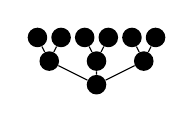
\begin{tikzpicture}[scale=.2]
    \node[circle, scale=0.75, fill] (tid0) at (4.5,1.5){};
    \node[circle, scale=0.75, fill] (tid1) at (1.5,3){};
    \node[circle, scale=0.75, fill] (tid4) at (0.75,4.5){};
    \node[circle, scale=0.75, fill] (tid5) at (2.25,4.5){};
    \draw[](tid1) -- (tid4);
    \draw[](tid1) -- (tid5);
    \node[circle, scale=0.75, fill] (tid2) at (4.5,3){};
    \node[circle, scale=0.75, fill] (tid6) at (3.75,4.5){};
    \node[circle, scale=0.75, fill] (tid7) at (5.25,4.5){};
    \draw[](tid2) -- (tid6);
    \draw[](tid2) -- (tid7);
    \node[circle, scale=0.75, fill] (tid3) at (7.5,3){};
    \node[circle, scale=0.75, fill] (tid8) at (6.75,4.5){};
    \node[circle, scale=0.75, fill] (tid9) at (8.25,4.5){};
    \draw[](tid3) -- (tid8);
    \draw[](tid3) -- (tid9);
    \draw[](tid0) -- (tid1);
    \draw[](tid0) -- (tid2);
    \draw[](tid0) -- (tid3);
  \end{tikzpicture}
\end{center}

However, we will most of the time use a notion where we assume that for a tree sequence $(x_1,x_2,\dots, x_n)$ we have $\forall i \in \left\{ 1,2,\dots,n \right\}x_i\leq i$. This is always possible because we can start a breadth-first search (BFS) at task 0 and assign numbers to the tasks representing the order in which BFS visits the tasks.

That means that there are $n!$ possibilities for tree sequences with exactly $n$ tasks. On the other hand, there are less (distinct) intrees of size $n$:

\begin{theorem}
  Let $T_n$ denote the number of intrees containing $n$ tasks. Then,
  \begin{equation*}
    T_n \sim C\cdot r^{-n}\cdot n^{-1.5} 
    \quad \text{ as } n\rightarrow \infty,
  \end{equation*}
  where $C=0.4399237\dots$ and $r=0.3383219\dots$.
\end{theorem}

\begin{proof}
  See \cite{asymptotic_enum_odlyzko}.
\end{proof}

The first values for $T_n$ are $0, 1, 1, 2, 4, 9, 20, 48, 115, 286, 719, 1842, 4766, 12486, 32973, \dots$ \cite{oeisrootedtrees}.

%\todo{Sollten auch andere Repräsentation erwähnt werden? We can represent an intree by a properly parenthesized expression, where leaves are denoted by 1 resp. 0 depending on whether they are scheduled resp. non-scheduled. We call the corresponding string the \emph{parenthesized expression} of an intree.}

\subsection{Interpretation as dependency graphs}
\label{sec:intrees-interpreted-as-dependency-graphs}

Those intrees can naturally be used to describe dependencies between different tasks, as long as each task is the requirement for \emph{at most one} other task. Each vertex in an intree then represents a task. If $t_1$ is a (direct) predecessor of $t_2$, this means that the task associated with $t_1$ must be executed before the task associated with $t_2$. Since we represent tasks by vertices, we will often use the terms task and vertex interchangeably.

\todo{Vielleicht ein Beispiel aus der echten Welt.}

\begin{definition}[Ready tasks]
  Let $I$ be an intree of tasks (represented by vertices) and. If $t$ is a leaf of $I$, we call the corresponding task (resp. -- for simplicity -- the whole vertex) \emph{ready}.
\end{definition}

The intree $(0,0,1,1,2,3,3,3,6,8)$ (see figure \ref{fig:intree-example-task-names-directed-edges}) has the ready tasks 4, 5, 7, 9 and 10.

\subsection{Labelled and unlabelled intrees}
\label{sec:intrees-labelled-unlabelled}

We can draw such intrees in a very straightforward manner: We draw the root at the bottom and its direct predecessors one level above. For each predecessor, we inductively repeat this procedure to obtain a ``top-to-bottom-description'' of the tree.

Figure \ref{fig:intree-example-task-names-directed-edges} shows an intree (the one given by the sequence $(0,0,1,1,2,3,3,3,6,8)$), where tasks 8 is a requirement for task 6, which itself is -- like task 7, 8 and (indirectly) task 10 -- a requirement for task 3. This figure also illustrates the fact that -- in an intree -- each task is a direct requirement for \emph{at most} one other task.

However, we are mostly interested in the \emph{structure} of the tree, which is why we most of the time omit the labellings of the vertices (i.e. we omit the task names) and rely on a \emph{unlabelled} representation as shown in figure \ref{fig:intree-example-structure-version}. 

\begin{figure}[t]
  \centering
  \begin{subfigure}{.45\textwidth}
    \centering{}
    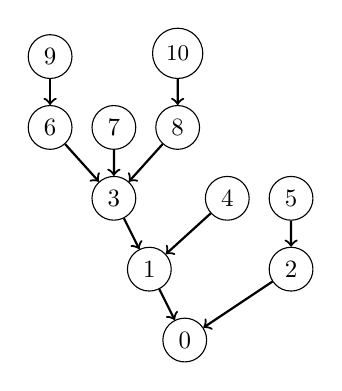
\begin{tikzpicture}[scale=.6, anchor=south]
      \node[circle, scale=0.9, draw] (tid0) at (3,1.5){0};
      \node[circle, scale=0.9, draw] (tid1) at (2.25,3){1};
      \node[circle, scale=0.9, draw] (tid2) at (1.5,4.5){3};
      \node[circle, scale=0.9, draw] (tid7) at (0.15,6){6};
      \node[circle, scale=0.9, draw] (tid9) at (0.15,7.5){9};
      \draw[<-, thick](tid7) -- (tid9);
      \node[circle, scale=0.9, draw] (tid10) at (1.5,6){7};
      \draw[<-, thick](tid2) -- (tid7);
      \draw[<-, thick](tid2) -- (tid10);
      \node[circle, scale=0.9, draw] (tid3) at (3.9,4.5){4};
      \node[circle, scale=0.9, draw] (tid5) at (2.85,6){8};
      \node[circle, scale=0.9, draw] (tid6) at (2.85,7.5){\small 10};
      \draw[<-, thick](tid5) -- (tid6);
      \draw[<-, thick](tid2) -- (tid5);
      \draw[<-, thick](tid1) -- (tid2);
      \draw[<-, thick](tid1) -- (tid3);
      \node[circle, scale=0.9, draw] (tid4) at (5.25,3){2};
      \node[circle, scale=0.9, draw] (tid8) at (5.25,4.5){5};
      \draw[<-, thick](tid4) -- (tid8);
      \draw[<-, thick](tid0) -- (tid1);
      \draw[<-, thick](tid0) -- (tid4);
    \end{tikzpicture}
    \caption{Labelled version with vertex labels and edges drawn as arrows.}
    \label{fig:intree-example-task-names-directed-edges}
  \end{subfigure}
  \quad
  \begin{subfigure}{.45\textwidth}
    \centering{}
    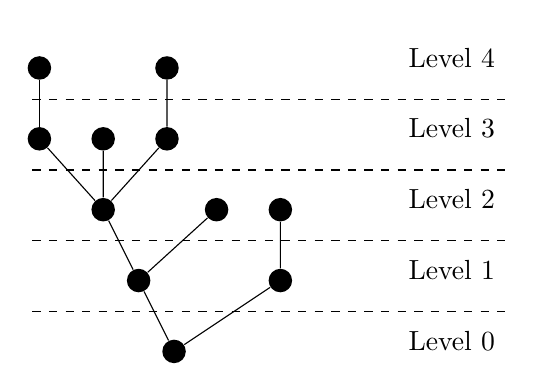
\begin{tikzpicture}[scale=.6, anchor=south]
      \node[circle, scale=0.9, fill] (tid0) at (3,1.5){};
      \node[circle, scale=0.9, fill] (tid1) at (2.25,3){};
      \node[circle, scale=0.9, fill] (tid2) at (1.5,4.5){};
      \node[circle, scale=0.9, fill] (tid7) at (0.15,6){};
      \node[circle, scale=0.9, fill] (tid9) at (0.15,7.5){};
      \draw[](tid7) -- (tid9);
      \node[circle, scale=0.9, fill] (tid10) at (1.5,6){};
      \draw[](tid2) -- (tid7);
      \draw[](tid2) -- (tid10);
      \node[circle, scale=0.9, fill] (tid3) at (3.9,4.5){};
      \node[circle, scale=0.9, fill] (tid5) at (2.85,6){};
      \node[circle, scale=0.9, fill] (tid6) at (2.85,7.5){};
      \draw[](tid5) -- (tid6);
      \draw[](tid2) -- (tid5);
      \draw[](tid1) -- (tid2);
      \draw[](tid1) -- (tid3);
      \node[circle, scale=0.9, fill] (tid4) at (5.25,3){};
      \node[circle, scale=0.9, fill] (tid8) at (5.25,4.5){};
      \draw[](tid4) -- (tid8);
      \draw[](tid0) -- (tid1);
      \draw[](tid0) -- (tid4);
      % level separators
      \draw[dashed] (0, 2.6) -- +(10, 0) node[below left, yshift=-.125cm]{Level 0};
      \draw[dashed] (0, 4.1) -- +(10, 0) node[below left, yshift=-.125cm]{Level 1};
      \draw[dashed] (0, 5.6) -- +(10, 0) node[below left, yshift=-.125cm]{Level 2};
      \draw[dashed] (0, 7.1) -- +(10, 0) node[below left, yshift=-.125cm]{Level 3};
      \draw[      ] (0, 8.6)    +(10, 0) node[below left, yshift=-.125cm]{Level 4};
    \end{tikzpicture}
    \caption{Unlabelled version without arrows, edges are implicitly directed towards the root.}
    \label{fig:intree-example-structure-version}
  \end{subfigure}
  \caption{Graphical representation of an intree ($(0,0,1,1,2,3,3,3,6,8)$) with 5 levels (numbered 0 to 4). All edges are implicitly directed towards the root, which is drawn at the bottom of the tree. Most of the time, the \emph{structure} of the tree is enough, so we will omit vertex names most of the time.}
  \label{fig:intrees-introductory-explanation}
\end{figure}

The mathematical concept behind unlabelled trees can be described by the notion of \emph{isomorphisms}.

\begin{definition}[Intree isomorphism]
  We call two intrees $I_1$ and $I_2$ \emph{isomorphic}, if there exists a bijective function that maps vertices of $I_1$ onto vertices of $I_2$ such that $(v,t)$ is an edge in $I_1$ if and only if $(f(v), f(t))$ is an edge in $I_2$ and the root of $I_1$ is mapped onto the root of $I_2$.
\end{definition}

\emph{Remark:} The above definition of isomorphisms is somwhat non-standard in the sense that usually isomorphisms are defined for undirected trees. For this work, we restrict ourselves onto our definition (except where explicitly stated otherwise).

As an example for isomorphic intrees, consider $(0,0,1,1,2,3,3,3,6,8)$, $(0,1,2,3,0,5,1,2,2,9)$ and $(0,1,0,3,3,4,4,7,4,9)$.

\subsection{Extension to in-forests}
\label{sec:intrees-extension-to-forests}

It is worth mentioning that -- for our needs -- there is a straightforward extension of intrees to in-forests for our scenario. In-forests are graphs whose components are all intrees. To convert an in-forest to an intree, we simply add an auxiliary new root and connect all roots of the intrees within the in-forest to the new root. This way, we clearly obtain a new intree.

\begin{figure}[th]
  \centering
  \begin{subfigure}{.45\textwidth}
    \centering
    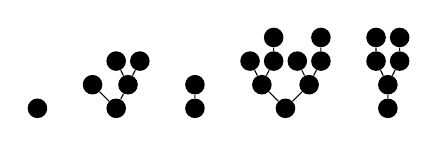
\begin{tikzpicture}[scale=.2, anchor=south]
      \begin{scope}[xshift=-2cm]
        \begin{scope}[xshift=-2cm]
          \node[circle, scale=0.75, fill] (tid1) at (0.75,3){};
        \end{scope}
        \node[circle, scale=0.75, fill] (tid2) at (3.75,3){};
        \node[circle, scale=0.75, fill] (tid6) at (2.25,4.5){};
        \node[circle, scale=0.75, fill] (tid7) at (4.5,4.5){};
        \node[circle, scale=0.75, fill] (tid12) at (3.75,6){};
        \node[circle, scale=0.75, fill] (tid13) at (5.25,6){};
      \end{scope}
      \draw[](tid7) -- (tid12);
      \draw[](tid7) -- (tid13);
      \draw[](tid2) -- (tid6);
      \draw[](tid2) -- (tid7);
      \node[circle, scale=0.75, fill] (tid3) at (6.75,3){};
      \node[circle, scale=0.75, fill] (tid8) at (6.75,4.5){};
      \draw[](tid3) -- (tid8);
      \begin{scope}[xshift=2cm]
        \node[circle, scale=0.75, fill] (tid4) at (10.5,3){};
        \node[circle, scale=0.75, fill] (tid9) at (9,4.5){};
        \node[circle, scale=0.75, fill] (tid14) at (8.25,6){};
        \node[circle, scale=0.75, fill] (tid15) at (9.75,6){};
        \node[circle, scale=0.75, fill] (tid20) at (9.75,7.5){};
        \draw[](tid15) -- (tid20);
        \draw[](tid9) -- (tid14);
        \draw[](tid9) -- (tid15);
        \node[circle, scale=0.75, fill] (tid10) at (12,4.5){};
        \node[circle, scale=0.75, fill] (tid16) at (11.25,6){};
        \node[circle, scale=0.75, fill] (tid17) at (12.75,6){};
        \node[circle, scale=0.75, fill] (tid21) at (12.75,7.5){};
        \draw[](tid17) -- (tid21);
        \draw[](tid10) -- (tid16);
        \draw[](tid10) -- (tid17);
        \draw[](tid4) -- (tid9);
        \draw[](tid4) -- (tid10);
        \begin{scope}[xshift=2cm]
          \node[circle, scale=0.75, fill] (tid5) at (15,3){};
          \node[circle, scale=0.75, fill] (tid11) at (15,4.5){};
          \node[circle, scale=0.75, fill] (tid18) at (14.25,6){};
          \node[circle, scale=0.75, fill] (tid22) at (14.25,7.5){};
          \draw[](tid18) -- (tid22);
          \node[circle, scale=0.75, fill] (tid19) at (15.75,6){};
          \node[circle, scale=0.75, fill] (tid23) at (15.75,7.5){};      
        \end{scope}
      \end{scope}
      \draw[](tid19) -- (tid23);
      \draw[](tid11) -- (tid18);
      \draw[](tid11) -- (tid19);
      \draw[](tid5) -- (tid11);
    \end{tikzpicture}
    \caption{Original in-forest (each component is a separate intree).}
  \end{subfigure}
  \quad
  \begin{subfigure}{.45\textwidth}
    \centering
    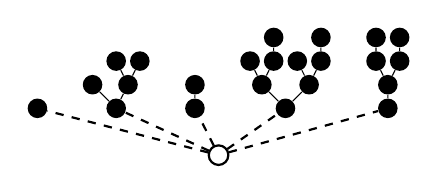
\begin{tikzpicture}[scale=.2, anchor=south]
      \node[circle, scale=0.75, draw, thick] (tid0) at (8.25,0){};
      \begin{scope}[xshift=-2cm]
        \begin{scope}[xshift=-2cm]
          \node[circle, scale=0.75, fill] (tid1) at (0.75,3){};
        \end{scope}
        \node[circle, scale=0.75, fill] (tid2) at (3.75,3){};
        \node[circle, scale=0.75, fill] (tid6) at (2.25,4.5){};
        \node[circle, scale=0.75, fill] (tid7) at (4.5,4.5){};
        \node[circle, scale=0.75, fill] (tid12) at (3.75,6){};
        \node[circle, scale=0.75, fill] (tid13) at (5.25,6){};
      \end{scope}
      \draw[](tid7) -- (tid12);
      \draw[](tid7) -- (tid13);
      \draw[](tid2) -- (tid6);
      \draw[](tid2) -- (tid7);
      \node[circle, scale=0.75, fill] (tid3) at (6.75,3){};
      \node[circle, scale=0.75, fill] (tid8) at (6.75,4.5){};
      \draw[](tid3) -- (tid8);
      \begin{scope}[xshift=2cm]
        \node[circle, scale=0.75, fill] (tid4) at (10.5,3){};
        \node[circle, scale=0.75, fill] (tid9) at (9,4.5){};
        \node[circle, scale=0.75, fill] (tid14) at (8.25,6){};
        \node[circle, scale=0.75, fill] (tid15) at (9.75,6){};
        \node[circle, scale=0.75, fill] (tid20) at (9.75,7.5){};
        \draw[](tid15) -- (tid20);
        \draw[](tid9) -- (tid14);
        \draw[](tid9) -- (tid15);
        \node[circle, scale=0.75, fill] (tid10) at (12,4.5){};
        \node[circle, scale=0.75, fill] (tid16) at (11.25,6){};
        \node[circle, scale=0.75, fill] (tid17) at (12.75,6){};
        \node[circle, scale=0.75, fill] (tid21) at (12.75,7.5){};
        \draw[](tid17) -- (tid21);
        \draw[](tid10) -- (tid16);
        \draw[](tid10) -- (tid17);
        \draw[](tid4) -- (tid9);
        \draw[](tid4) -- (tid10);
        \begin{scope}[xshift=2cm]
          \node[circle, scale=0.75, fill] (tid5) at (15,3){};
          \node[circle, scale=0.75, fill] (tid11) at (15,4.5){};
          \node[circle, scale=0.75, fill] (tid18) at (14.25,6){};
          \node[circle, scale=0.75, fill] (tid22) at (14.25,7.5){};
          \draw[](tid18) -- (tid22);
          \node[circle, scale=0.75, fill] (tid19) at (15.75,6){};
          \node[circle, scale=0.75, fill] (tid23) at (15.75,7.5){};      
        \end{scope}
      \end{scope}
      \draw[](tid19) -- (tid23);
      \draw[](tid11) -- (tid18);
      \draw[](tid11) -- (tid19);
      \draw[](tid5) -- (tid11);
      \draw[dashed, thick](tid0) -- (tid1);
      \draw[dashed, thick](tid0) -- (tid2);
      \draw[dashed, thick](tid0) -- (tid3);
      \draw[dashed, thick](tid0) -- (tid4);
      \draw[dashed, thick](tid0) -- (tid5);
    \end{tikzpicture}
    \caption{Adding a new root that is connected with all intrees' roots.}
  \end{subfigure}
  \caption{Converting an in-forest to an intree.}
  \label{fig:in-forest-to-intree}
\end{figure}

To manipulate intrees, we define some non-standard notation that is, however, very convenient and should be easily understandable.

\section{Schedules}
\label{sec:introduction-schedules}

We will now combine the knowledge from sections \ref{sec:some-probability} and \ref{sec:foundations-graph-theory} and introduce the structure we will be working on. 

\subsection{Computational setting \todo{Better title.}}
\label{sec:schedules-problem-setting}

We now describe our assumptions concerning the tasks to be processed and our machines.

\paragraph{Intree constraint}

We assume that the dependencies between the tasks under consideration can be described as an intree (as introduced in  section \ref{sec:foundations-graph-theory}).

\paragraph{Random task processing times}

We assume that we do not know the processing time for a certain task in advance. We instead assume that we can model the task time for each task within the intree by an exponentially distributed random variable as defined in section \ref{sec:exponential-distribution}. We furthermore assume that all tasks are exponentially distributed with the \emph{same} parameter $\lambda$. Note that we can assume w.l.o.g. --  according to theorem \ref{thm:expoenential-distr-scalability} explaining exponential variables' scaling -- that all tasks have parameter $\lambda=1$.

\paragraph{Parallel processors}

We assume that we have a certain number (we will focus on 2 or 3) of \emph{identical} processors. These processors work in parallel and can be used to carry out the individual tasks. For simplicity we assume that switching from one task to another takes no time at all.

\paragraph{Tasks are ``atomic''}

We assume that one single task can be processed by one processor exclusively, i.e. it is not possible to save time by ``splitting'' one single task over several processors. That, moreover, means that there might be idle processors if we have more ready tasks than processors.

\paragraph{Non-preemtive scheduling}

We will focus on non-preemtive scheduling, i.e. once a task is processor is assigned a task, this task has to be processed \emph{completely} before the processor can be used for anything else. Note that the restriction on non-preemtive scheduling is no problem when we work with two processors (as shown in \cite{chandyreynoldslargepaper1979}) --- in this case, the optimal schedule is (without loss of generality) non-preemtive. However, for three processors, preemtive schedules might be better than non-preemtive ones. We will later show an example intree for this fact (see section \ref{preemtiveness-explanation}).

However, as shown in \cite{chandyreynoldslargepaper1979} an optimal schedule (without loss of generality) only preemts a task directly after another task finishes.

\subsection{Processing a whole intree of tasks}
\label{sec:processing-an-intree-of-tasks}

Assuming that we have a certain amount $p$ of identical processors, we can process all tasks in an intree (of course in a valid order). Naturally, We have to do this step by step. 

That is, we assign some (at most $p$) ready tasks to processors, wait until the first assigned task finishes, assign a new task (if available) to the now idle processor, and continue with the subtree obtained by removing the finished task. That is, in each point of time, we know the current intree containing all tasks not yet finished and all tasks currently being processed. We therefore introduce the notation of \emph{snapshots}.

\begin{definition}[Schedules and snapshots]  
  Let $I$ be an intree of tasks that is processed. A \emph{schedule} is the order in which tasks are processed. Since task times are unknown, this order is not deterministic and can vary from execution to execution.

  Let $S$ be a schedule of $I$.
  A \emph{snapshot} of $S$ a pair containing
  \begin{itemize}
  \item the current subtree $I'\subseteq I$ describing which tasks are not finished yet,
  \item a set $X$ holding the tasks that are currently being processed (i.e. a set of \emph{currently scheduled tasks}).
  \end{itemize}
\end{definition}

While the above definition is well suited for theoretical considerations, we -- most of the time -- are satisfied with a concise graphical representation, that will look as shown in figure \ref{fig:intro-snapshot-graphical-representation}, i.e. it is depicted as an intree, whose scheduled tasks are marked by a cross\todo{Schauen, ob ich das geändert habe!}.

\begin{figure}[t]
  \centering
  \begin{tikzpicture}[scale=.2, anchor=south]
    \node[circle, scale=0.75, fill] (tid0) at (3,1.5){};
    \node[circle, scale=0.75, fill] (tid1) at (1.5,3){};
    \node[circle, scale=0.75, fill] (tid3) at (0.75,4.5){};
    \node[circle, scale=0.75, fill] (tid4) at (2.25,4.5){};
    \node[circle, scale=0.75, fill, task_scheduled] (tid7) at (2.25,6){};
    \draw[](tid4) -- (tid7);
    \draw[](tid1) -- (tid3);
    \draw[](tid1) -- (tid4);
    \node[circle, scale=0.75, fill] (tid2) at (3.75,3){};
    \node[circle, scale=0.75, fill] (tid5) at (5.25,3){};
    \node[circle, scale=0.75, fill, task_scheduled] (tid6) at (5.25,4.5){};
    \draw[](tid5) -- (tid6);
    \draw[](tid0) -- (tid1);
    \draw[](tid0) -- (tid2);
    \draw[](tid0) -- (tid5);
    % arrows for scheduled tasks
    \draw(tid7) +(1,0)[<-, thick] ..controls+(4,0) and +(0,1).. (15,3);
    \draw(tid6) +(1,0)[<-, thick] ..controls+(2,0) and +(0,1).. (15,3) 
    node[below]{scheduled tasks};
    % brace for whole intree
    \draw[decorate, decoration=brace](-1,1) --node[left, xshift=-.1cm]{current intree} +(0,7);
  \end{tikzpicture}
  \caption{A snapshot is determined by its intree and a collection of currently scheduled tasks.}
  \label{fig:intro-snapshot-graphical-representation}
\end{figure}

Consider now a snapshot, i.e. the current intree and a set of currently scheduled tasks. At this point, there are several possibilities:

\begin{itemize}
\item Any of the currently scheduled tasks may be the first task to finish.
\item If a certain task finishes, the corresponding processor gets idle and can be assigned new work. That is, we may be able to choose a new task\footnote{It may be the case that we are not able to select any new task because all leaves are already scheduled. In this case, the processor has to stay idle and can not get assigned a new task.} and assign it to the now idle processor.

  Note that we can -- in principle -- easily choose a certain task with some probability and another task with another probability, thus introducing more possibilities.
\end{itemize}

That is, we have several possibilities here. The first of them (which task finishes first) can not be influenced in our scenario. The second, however, leaves us a choice that we can influence. Depending on which task we choose next, we might get a better or worse overall run time.

\begin{definition}[Scheduling strategy]
  A \emph{scheduling strategy} determines the probability that a certai tasks should be the next tasks to be scheduled.
\end{definition}

That means, we use the notion of a \emph{probabilistic scheduler} in the sense that the scheduler is not forced to restrict on \emph{one single} task, but can instead specify probabilities for each ready, currently unscheduled task. Note that we can easily ``simulate'' a deterministic scheduler by assigning probability 1 to one single ready task, and probability 0 to all other possibilities.

One desirable goal is to always choose the next task to be scheduled (resp. the respective probabilities) in such a way that the overall expected run time is minimal. We will now see how we can compute the expected run time for a schedule.

\subsection{Two prominent scheduling strategies}
\label{sec:intro-two-scheduling-strategies}

We will now present two important scheduling strategies that we will use to research the problem throughout this work.

\begin{definition}[HLF scheduling]
  A \emph{highest level first} scheduler (or HLF scheduler) assigns, if there are idle processors, ready tasks whose levels are maximal.
\end{definition}

Note that the above definition of HLF leaves some freedom if there are several tasks that could be chosen by HLF. If this is the case, then there are (basically) two possibilities:
\begin{itemize}
\item Choose \emph{one} task according to a certain pattern or randomly.
\item Assign to \emph{each} possibly chosen task a certain probability.
\end{itemize}

Note that we can consider the first possibility as a special case of the second one. HLF scheduling is optimal for intrees whose task times are equal scheduled on any number of processors \cite{hu:1961:hlfoptimalforknowntimesintree} and for intrees whose task times are exponentially distributed (with same parameter) scheduled on two processors (see \cite{chandyreynoldsshortpaper1975} and chapter \ref{chap:p2}). 

Another (very trivial) scheduler is the scheduler that tries all possibilities:

\begin{definition}[LEAF scheduling]
  A LEAF scheduler, if a processor gets free and can be assigned a new task, assigns each ready task with the same probability to this processor. In the beginning, each possible combination of scheduled tasks is taken with the same probability.
\end{definition}

LEAF schedulers are useful to examine all possible schedules and play an important role when we research how many snapshots have to be examined \emph{at most}.

\subsection{Visualizing a schedule}
\label{sec:intro-visualizing-schedules}

If we are speaking of a schedule, we talk about the complete processing of an intree of tasks.

We can think of it as a connected directed acyclic graph or DAG (see \cite{diestel2005graph} for more information), where each vertex represents one single snapshot. The edges between the snapshots then represent transitions that indicate that a certain task has finished and (possibly) a new task has chosen to be scheduled. We can naturally assign the edges weights that represent the corresponding probability that a task has finished and the new task has been picked.

As stated before, we have two sources of non-determinism:
\begin{itemize}
\item Each of the currently scheduled tasks can be the first task to finish. Depending on which task finishes first, we have to continue with another intree.
\item When one task finishes, the corresponding processor becomes idle and can be used to process other tasks. This is the second source where we have different possibilities. However, for this point, we can decide ourselves how to continue.
\end{itemize}

We will look at the intree $(0,0,1,2,2,2,6,6,8)$ -- it shall be processed by two processors -- as an example. This intree looks as follows:

\begin{center}
  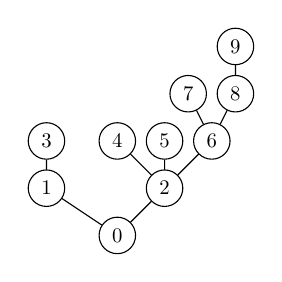
\begin{tikzpicture}[scale=.4]
    \node[circle, scale=0.75, draw] (tid0) at (4.5,1.5){0};
    \node[circle, scale=0.75, draw] (tid2) at (2.25,3){1};
    \node[circle, scale=0.75, draw] (tid4) at (2.25,4.5){3};
    \draw[](tid2) -- (tid4);
    \node[circle, scale=0.75, draw] (tid3) at (6,3){2};
    \node[circle, scale=0.75, draw] (tid5) at (4.5,4.5){4};
    \node[circle, scale=0.75, draw] (tid6) at (6,4.5){5};
    \node[circle, scale=0.75, draw] (tid7) at (7.5,4.5){6};
    \node[circle, scale=0.75, draw] (tid8) at (6.75,6){7};
    \node[circle, scale=0.75, draw] (tid9) at (8.25,6){8};
    \node[circle, scale=0.75, draw] (tid10) at (8.25,7.5){9};
    \draw[](tid9) -- (tid10);
    \draw[](tid7) -- (tid8);
    \draw[](tid7) -- (tid9);
    \draw[](tid3) -- (tid5);
    \draw[](tid3) -- (tid6);
    \draw[](tid3) -- (tid7);
    \draw[](tid0) -- (tid2);
    \draw[](tid0) -- (tid3);
  \end{tikzpicture}
\end{center}

Figure \ref{fig:schedule-dag-intro} shows (the beginning) a two-processor schedule for the intree $(0,0,1,2,2,2,6.6,8)$ in two variants: Figure \ref{fig:schedule-dag-intro-intermediates} shows the schedule and incorporates situations where the scheduler can decide wich tasks should be scheduled next with wich probabilities (``intermediate snapshots''). At the beginning, the nodes 9 and 3 are scheduled (snapshot $A$). Then each of these two tasks is the first one to finish (each one with probability 50\%). This intermediate situation, where exactly one of the two tasks is finished and the scheduler can assign probabilities describing which task to pick next, are shown in snapshots $B$ (this is the situation where task 3 finished first) and $C$ (where 9 finished first).

In the situation described by the intermediate snapshot $B$, the scheduler can decide which task shall be chosen next with which probability. In the situation of snapshot $B$, the scheduler decides that with probability 20\%, the task 1 shall be chosen as next task (snapshot $B_1$) and with probability 80\% task 4 shall be chosen as next task (snapshot $B_2$). Similarily it decides in the situation denoted by $C$ that tasks 8 resp. 4 shall be chosen with probability 40\% each ($C_1$ resp. $C_3$) and task 7 shall be chosen with probability 20\% ($C_2$).

\begin{figure}[th]
  \centering
  \begin{subfigure}{\textwidth}
    \centering
    \renewcommand{\leveltopI}{-12cm + \leveltop}
\renewcommand{\leveltopII}{-12cm + \leveltopI}
\renewcommand{\leveltopIII}{-14cm + \leveltopII}
\renewcommand{\leveltopIIII}{-12cm + \leveltopIII}
\renewcommand{\leveltopIIIII}{-12cm + \leveltopIIII}
\renewcommand{\leveltopIIIIII}{-12cm + \leveltopIIIII}
\renewcommand{\leveltopIIIIIII}{-12cm + \leveltopIIIIII}
\renewcommand{\leveltopIIIIIIII}{-12cm + \leveltopIIIIIII}
\renewcommand{\leveltopIIIIIIIII}{-12cm + \leveltopIIIIIIII}
\renewcommand{\leveltopIIIIIIIIII}{-12cm + \leveltopIIIIIIIII}
\renewcommand{\leveltopIIIIIIIIIII}{-12cm + \leveltopIIIIIIIIII}
\begin{tikzpicture}[scale=.2, anchor=south]
  % "key"
  \fill[fill=gray!10!white] (-35, -24) rectangle +(72, 9.5);
  \draw[dashed] (-35, -14.5) -- +(72, 0);
  \draw[dashed] (-35, -24) -- +(72, 0);
  \node at (27, -21) {Intermediate snapshots};
  \begin{scope}[yshift=\leveltopI cm]
    \node at (-7.5,3) {\huge $A$};
    \matrix (line1)[column sep=0.5cm] {
      \node[draw=black, rectangle split,  rectangle split parts=1] (sn0x17d67b0){
        \begin{tikzpicture}[scale=.2]
          \node[circle, scale=0.75, fill] (tid0) at (4.5,1.5){};
          \node[circle, scale=0.75, fill] (tid2) at (2.25,3){};
          \node[circle, scale=0.75, fill, task_scheduled] (tid4) at (2.25,4.5){};
          \draw[](tid2) -- (tid4);
          \node[circle, scale=0.75, fill] (tid3) at (6,3){};
          \node[circle, scale=0.75, fill] (tid5) at (3.75,4.5){};
          \node[circle, scale=0.75, fill] (tid6) at (5.25,4.5){};
          \node[circle, scale=0.75, fill] (tid7) at (7.5,4.5){};
          \node[circle, scale=0.75, fill] (tid8) at (6.75,6){};
          \node[circle, scale=0.75, fill] (tid9) at (8.25,6){};
          \node[circle, scale=0.75, fill, task_scheduled] (tid10) at (8.25,7.5){};
          \draw[](tid9) -- (tid10);
          \draw[](tid7) -- (tid8);
          \draw[](tid7) -- (tid9);
          \draw[](tid3) -- (tid5);
          \draw[](tid3) -- (tid6);
          \draw[](tid3) -- (tid7);
          \draw[](tid0) -- (tid2);
          \draw[](tid0) -- (tid3);
        \end{tikzpicture}
      };
      & 
      \\
    };
  \end{scope}
  \begin{scope}[yshift=\leveltopII cm]
    \matrix (line2)[column sep=0.5cm] {
      \node[draw=black, rectangle split,  rectangle split parts=1] (sn0x17d65a0){
        \begin{tikzpicture}[scale=.2]
          \node[circle, scale=0.75, fill] (tid0) at (4.5,1.5){};
          \node[circle, scale=0.75, fill] (tid2) at (2.25,3){};
          \node[circle, scale=0.75, fill] (tid3) at (6,3){};
          \node[circle, scale=0.75, fill] (tid5) at (3.75,4.5){};
          \node[circle, scale=0.75, fill] (tid6) at (5.25,4.5){};
          \node[circle, scale=0.75, fill] (tid7) at (7.5,4.5){};
          \node[circle, scale=0.75, fill] (tid8) at (6.75,6){};
          \node[circle, scale=0.75, fill] (tid9) at (8.25,6){};
          \node[circle, scale=0.75, fill, task_scheduled] (tid10) at (8.25,7.5){};
          \draw[](tid9) -- (tid10);
          \draw[](tid7) -- (tid8);
          \draw[](tid7) -- (tid9);
          \draw[](tid3) -- (tid5);
          \draw[](tid3) -- (tid6);
          \draw[](tid3) -- (tid7);
          \draw[](tid0) -- (tid2);
          \draw[](tid0) -- (tid3);
        \end{tikzpicture}
      }
      node[left, xshift=-25, yshift=25]{\huge $B$};
      & 
      \node[minimum width=1cm]{};
      &
      \node[draw=black, rectangle split,  rectangle split parts=1] (sn0x17d57c0){
        \begin{tikzpicture}[scale=.2]
          \node[circle, scale=0.75, fill] (tid0) at (4.5,1.5){};
          \node[circle, scale=0.75, fill] (tid2) at (2.25,3){};
          \node[circle, scale=0.75, fill, task_scheduled] (tid4) at (2.25,4.5){};
          \draw[](tid2) -- (tid4);
          \node[circle, scale=0.75, fill] (tid3) at (6,3){};
          \node[circle, scale=0.75, fill] (tid5) at (3.75,4.5){};
          \node[circle, scale=0.75, fill] (tid6) at (5.25,4.5){};
          \node[circle, scale=0.75, fill] (tid7) at (7.5,4.5){};
          \node[circle, scale=0.75, fill] (tid8) at (6.75,6){};
          \node[circle, scale=0.75, fill] (tid9) at (8.25,6){};
          \draw[](tid7) -- (tid8);
          \draw[](tid7) -- (tid9);
          \draw[](tid3) -- (tid5);
          \draw[](tid3) -- (tid6);
          \draw[](tid3) -- (tid7);
          \draw[](tid0) -- (tid2);
          \draw[](tid0) -- (tid3);
        \end{tikzpicture}
      }
      node[left, xshift=-25, yshift=25]{\huge $C$};
      & 
      \\
    };
  \end{scope}
  \begin{scope}[yshift=\leveltopIII cm]
    \matrix (line3)[column sep=0.5cm] {
      \node[draw=black, rectangle split,  rectangle split parts=1] (sn0x17d55b0){
        \begin{tikzpicture}[scale=.2]
          \node[circle, scale=0.75, fill] (tid0) at (4.5,1.5){};
          \node[circle, scale=0.75, fill, task_scheduled] (tid2) at (2.25,3){};
          \node[circle, scale=0.75, fill] (tid3) at (6,3){};
          \node[circle, scale=0.75, fill] (tid5) at (3.75,4.5){};
          \node[circle, scale=0.75, fill] (tid6) at (5.25,4.5){};
          \node[circle, scale=0.75, fill] (tid7) at (7.5,4.5){};
          \node[circle, scale=0.75, fill] (tid8) at (6.75,6){};
          \node[circle, scale=0.75, fill] (tid9) at (8.25,6){};
          \node[circle, scale=0.75, fill, task_scheduled] (tid10) at (8.25,7.5){};
          \draw[](tid9) -- (tid10);
          \draw[](tid7) -- (tid8);
          \draw[](tid7) -- (tid9);
          \draw[](tid3) -- (tid5);
          \draw[](tid3) -- (tid6);
          \draw[](tid3) -- (tid7);
          \draw[](tid0) -- (tid2);
          \draw[](tid0) -- (tid3);
        \end{tikzpicture}
      }
      node[left, xshift=-25, yshift=25]{\huge $B_1$};
      & 
      \node[draw=black, rectangle split,  rectangle split parts=1] (sn0x17d6160){
        \begin{tikzpicture}[scale=.2]
          \node[circle, scale=0.75, fill] (tid0) at (4.5,1.5){};
          \node[circle, scale=0.75, fill] (tid2) at (2.25,3){};
          \node[circle, scale=0.75, fill] (tid3) at (6,3){};
          \node[circle, scale=0.75, fill, task_scheduled] (tid5) at (3.75,4.5){};
          \node[circle, scale=0.75, fill] (tid6) at (5.25,4.5){};
          \node[circle, scale=0.75, fill] (tid7) at (7.5,4.5){};
          \node[circle, scale=0.75, fill] (tid8) at (6.75,6){};
          \node[circle, scale=0.75, fill] (tid9) at (8.25,6){};
          \node[circle, scale=0.75, fill, task_scheduled] (tid10) at (8.25,7.5){};
          \draw[](tid9) -- (tid10);
          \draw[](tid7) -- (tid8);
          \draw[](tid7) -- (tid9);
          \draw[](tid3) -- (tid5);
          \draw[](tid3) -- (tid6);
          \draw[](tid3) -- (tid7);
          \draw[](tid0) -- (tid2);
          \draw[](tid0) -- (tid3);
        \end{tikzpicture}
      }
      node[left, xshift=-25, yshift=25]{\huge $B_2$};
      & 
      \node[draw=black, rectangle split,  rectangle split parts=1] (sn0x17d5380){
        \begin{tikzpicture}[scale=.2]
          \node[circle, scale=0.75, fill] (tid0) at (4.5,1.5){};
          \node[circle, scale=0.75, fill] (tid2) at (2.25,3){};
          \node[circle, scale=0.75, fill, task_scheduled] (tid4) at (2.25,4.5){};
          \draw[](tid2) -- (tid4);
          \node[circle, scale=0.75, fill] (tid3) at (6,3){};
          \node[circle, scale=0.75, fill] (tid5) at (3.75,4.5){};
          \node[circle, scale=0.75, fill] (tid6) at (5.25,4.5){};
          \node[circle, scale=0.75, fill] (tid7) at (7.5,4.5){};
          \node[circle, scale=0.75, fill] (tid8) at (6.75,6){};
          \node[circle, scale=0.75, fill, task_scheduled] (tid9) at (8.25,6){};
          \draw[](tid7) -- (tid8);
          \draw[](tid7) -- (tid9);
          \draw[](tid3) -- (tid5);
          \draw[](tid3) -- (tid6);
          \draw[](tid3) -- (tid7);
          \draw[](tid0) -- (tid2);
          \draw[](tid0) -- (tid3);
        \end{tikzpicture}
      }
      node[left, xshift=-25, yshift=25]{\huge $C_1$};
      & 
      \node[draw=black, rectangle split,  rectangle split parts=1] (sn0x17d2f50){
        \begin{tikzpicture}[scale=.2]
          \node[circle, scale=0.75, fill] (tid0) at (4.5,1.5){};
          \node[circle, scale=0.75, fill] (tid2) at (2.25,3){};
          \node[circle, scale=0.75, fill, task_scheduled] (tid4) at (2.25,4.5){};
          \draw[](tid2) -- (tid4);
          \node[circle, scale=0.75, fill] (tid3) at (6,3){};
          \node[circle, scale=0.75, fill] (tid5) at (3.75,4.5){};
          \node[circle, scale=0.75, fill] (tid6) at (5.25,4.5){};
          \node[circle, scale=0.75, fill] (tid7) at (7.5,4.5){};
          \node[circle, scale=0.75, fill, task_scheduled] (tid8) at (6.75,6){};
          \node[circle, scale=0.75, fill] (tid9) at (8.25,6){};
          \draw[](tid7) -- (tid8);
          \draw[](tid7) -- (tid9);
          \draw[](tid3) -- (tid5);
          \draw[](tid3) -- (tid6);
          \draw[](tid3) -- (tid7);
          \draw[](tid0) -- (tid2);
          \draw[](tid0) -- (tid3);
        \end{tikzpicture}
      }
      node[left, xshift=-25, yshift=25]{\huge $C_2$};
      & 
      \node[draw=black, rectangle split,  rectangle split parts=1] (sn0x17d3a00){
        \begin{tikzpicture}[scale=.2]
          \node[circle, scale=0.75, fill] (tid0) at (4.5,1.5){};
          \node[circle, scale=0.75, fill] (tid2) at (2.25,3){};
          \node[circle, scale=0.75, fill, task_scheduled] (tid4) at (2.25,4.5){};
          \draw[](tid2) -- (tid4);
          \node[circle, scale=0.75, fill] (tid3) at (6,3){};
          \node[circle, scale=0.75, fill, task_scheduled] (tid5) at (3.75,4.5){};
          \node[circle, scale=0.75, fill] (tid6) at (5.25,4.5){};
          \node[circle, scale=0.75, fill] (tid7) at (7.5,4.5){};
          \node[circle, scale=0.75, fill] (tid8) at (6.75,6){};
          \node[circle, scale=0.75, fill] (tid9) at (8.25,6){};
          \draw[](tid7) -- (tid8);
          \draw[](tid7) -- (tid9);
          \draw[](tid3) -- (tid5);
          \draw[](tid3) -- (tid6);
          \draw[](tid3) -- (tid7);
          \draw[](tid0) -- (tid2);
          \draw[](tid0) -- (tid3);
        \end{tikzpicture}
      }
      node[left, xshift=-25, yshift=25]{\huge $C_3$};
      & 
      \\
    };
  \end{scope}
  \draw (sn0x17d67b0.south) -- node[xshift=.4cm]{$0.5$} (sn0x17d57c0.north);
  \draw (sn0x17d67b0.south) -- node[left, xshift=-.4cm]{$0.5$} (sn0x17d65a0.north);
  \draw (sn0x17d65a0.south) -- node[right, xshift=.25cm]{$0.8$} (sn0x17d6160.north);
  \draw (sn0x17d65a0.south) -- node[left, xshift=-.25cm]{$0.2$} (sn0x17d55b0.north);
  \draw (sn0x17d57c0.south) -- node[right, xshift=.25]{$0.2$} (sn0x17d2f50.north);
  \draw (sn0x17d57c0.south) -- node[xshift=-.5]{$0.4$} (sn0x17d5380.north);
  \draw (sn0x17d57c0.south) -- node[right, xshift=.25]{$0.4$} (sn0x17d3a00.north);
\end{tikzpicture}
%%% Local Variables:
%%% TeX-master: "thesis/thesis.tex"
%%% End: 

    \caption{A snapshot DAG with intermediate snapshots. In the beginning, there are two tasks scheduled. Each task is the first to finish with probability 0.5 (see the corresponding edges). An intermediate snapshot describes a situation where the scheduler can assign probabilities to be scheduled as next task to the tasks. According to these probabilities, the processing continues with the corresponding probabilities.}
  \label{fig:schedule-dag-intro-intermediates}
  \end{subfigure}
  \begin{subfigure}{\textwidth}
    \centering
    \renewcommand{\leveltopI}{-12cm + \leveltop}
\renewcommand{\leveltopII}{-10cm + \leveltopI}
\renewcommand{\leveltopIII}{-10cm + \leveltopII}
\renewcommand{\leveltopIIII}{-12cm + \leveltopIII}
\renewcommand{\leveltopIIIII}{-12cm + \leveltopIIII}
\renewcommand{\leveltopIIIIII}{-12cm + \leveltopIIIII}
\renewcommand{\leveltopIIIIIII}{-12cm + \leveltopIIIIII}
\renewcommand{\leveltopIIIIIIII}{-12cm + \leveltopIIIIIII}
\renewcommand{\leveltopIIIIIIIII}{-12cm + \leveltopIIIIIIII}
\renewcommand{\leveltopIIIIIIIIII}{-12cm + \leveltopIIIIIIIII}
\renewcommand{\leveltopIIIIIIIIIII}{-12cm + \leveltopIIIIIIIIII}
\begin{tikzpicture}[scale=.13333, anchor=south]
  \begin{scope}[yshift=\leveltopI cm]
    \matrix (line1)[column sep=0.5cm] {
      \node[draw=black, rectangle split,  rectangle split parts=2] (sn0x17d67b0){
        \begin{tikzpicture}[scale=.13333]
          \node[circle, scale=0.5, fill] (tid0) at (4.5,1.5){};
          \node[circle, scale=0.5, fill] (tid2) at (2.25,3){};
          \node[circle, scale=0.5, fill, task_scheduled] (tid4) at (2.25,4.5){};
          \draw[](tid2) -- (tid4);
          \node[circle, scale=0.5, fill] (tid3) at (6,3){};
          \node[circle, scale=0.5, fill] (tid5) at (3.75,4.5){};
          \node[circle, scale=0.5, fill] (tid6) at (5.25,4.5){};
          \node[circle, scale=0.5, fill] (tid7) at (7.5,4.5){};
          \node[circle, scale=0.5, fill] (tid8) at (6.75,6){};
          \node[circle, scale=0.5, fill] (tid9) at (8.25,6){};
          \node[circle, scale=0.5, fill, task_scheduled] (tid10) at (8.25,7.5){};
          \draw[](tid9) -- (tid10);
          \draw[](tid7) -- (tid8);
          \draw[](tid7) -- (tid9);
          \draw[](tid3) -- (tid5);
          \draw[](tid3) -- (tid6);
          \draw[](tid3) -- (tid7);
          \draw[](tid0) -- (tid2);
          \draw[](tid0) -- (tid3);
        \end{tikzpicture}
        \nodepart{two}
        \footnotesize{10\ 40\ 20\ 10\ 20}
      };
      & 
      \\
    };
  \end{scope}
  \begin{scope}[yshift=\leveltopII cm]
    \matrix (line3)[column sep=0.5cm] {
      \node[draw=black, rectangle split,  rectangle split parts=1] (sn0x17d55b0){
        \begin{tikzpicture}[scale=.13333]
          \node[circle, scale=0.5, fill] (tid0) at (4.5,1.5){};
          \node[circle, scale=0.5, fill, task_scheduled] (tid2) at (2.25,3){};
          \node[circle, scale=0.5, fill] (tid3) at (6,3){};
          \node[circle, scale=0.5, fill] (tid5) at (3.75,4.5){};
          \node[circle, scale=0.5, fill] (tid6) at (5.25,4.5){};
          \node[circle, scale=0.5, fill] (tid7) at (7.5,4.5){};
          \node[circle, scale=0.5, fill] (tid8) at (6.75,6){};
          \node[circle, scale=0.5, fill] (tid9) at (8.25,6){};
          \node[circle, scale=0.5, fill, task_scheduled] (tid10) at (8.25,7.5){};
          \draw[](tid9) -- (tid10);
          \draw[](tid7) -- (tid8);
          \draw[](tid7) -- (tid9);
          \draw[](tid3) -- (tid5);
          \draw[](tid3) -- (tid6);
          \draw[](tid3) -- (tid7);
          \draw[](tid0) -- (tid2);
          \draw[](tid0) -- (tid3);
        \end{tikzpicture}
      };
      & 
      \node[draw=black, rectangle split,  rectangle split parts=1] (sn0x17d6160){
        \begin{tikzpicture}[scale=.13333]
          \node[circle, scale=0.5, fill] (tid0) at (4.5,1.5){};
          \node[circle, scale=0.5, fill] (tid2) at (2.25,3){};
          \node[circle, scale=0.5, fill] (tid3) at (6,3){};
          \node[circle, scale=0.5, fill, task_scheduled] (tid5) at (3.75,4.5){};
          \node[circle, scale=0.5, fill] (tid6) at (5.25,4.5){};
          \node[circle, scale=0.5, fill] (tid7) at (7.5,4.5){};
          \node[circle, scale=0.5, fill] (tid8) at (6.75,6){};
          \node[circle, scale=0.5, fill] (tid9) at (8.25,6){};
          \node[circle, scale=0.5, fill, task_scheduled] (tid10) at (8.25,7.5){};
          \draw[](tid9) -- (tid10);
          \draw[](tid7) -- (tid8);
          \draw[](tid7) -- (tid9);
          \draw[](tid3) -- (tid5);
          \draw[](tid3) -- (tid6);
          \draw[](tid3) -- (tid7);
          \draw[](tid0) -- (tid2);
          \draw[](tid0) -- (tid3);
        \end{tikzpicture}
      };
      & 
      \node[draw=black, rectangle split,  rectangle split parts=1] (sn0x17d5380){
        \begin{tikzpicture}[scale=.13333]
          \node[circle, scale=0.5, fill] (tid0) at (4.5,1.5){};
          \node[circle, scale=0.5, fill] (tid2) at (2.25,3){};
          \node[circle, scale=0.5, fill, task_scheduled] (tid4) at (2.25,4.5){};
          \draw[](tid2) -- (tid4);
          \node[circle, scale=0.5, fill] (tid3) at (6,3){};
          \node[circle, scale=0.5, fill] (tid5) at (3.75,4.5){};
          \node[circle, scale=0.5, fill] (tid6) at (5.25,4.5){};
          \node[circle, scale=0.5, fill] (tid7) at (7.5,4.5){};
          \node[circle, scale=0.5, fill] (tid8) at (6.75,6){};
          \node[circle, scale=0.5, fill, task_scheduled] (tid9) at (8.25,6){};
          \draw[](tid7) -- (tid8);
          \draw[](tid7) -- (tid9);
          \draw[](tid3) -- (tid5);
          \draw[](tid3) -- (tid6);
          \draw[](tid3) -- (tid7);
          \draw[](tid0) -- (tid2);
          \draw[](tid0) -- (tid3);
        \end{tikzpicture}
      };
      & 
      \node[draw=black, rectangle split,  rectangle split parts=1] (sn0x17d2f50){
        \begin{tikzpicture}[scale=.13333]
          \node[circle, scale=0.5, fill] (tid0) at (4.5,1.5){};
          \node[circle, scale=0.5, fill] (tid2) at (2.25,3){};
          \node[circle, scale=0.5, fill, task_scheduled] (tid4) at (2.25,4.5){};
          \draw[](tid2) -- (tid4);
          \node[circle, scale=0.5, fill] (tid3) at (6,3){};
          \node[circle, scale=0.5, fill] (tid5) at (3.75,4.5){};
          \node[circle, scale=0.5, fill] (tid6) at (5.25,4.5){};
          \node[circle, scale=0.5, fill] (tid7) at (7.5,4.5){};
          \node[circle, scale=0.5, fill, task_scheduled] (tid8) at (6.75,6){};
          \node[circle, scale=0.5, fill] (tid9) at (8.25,6){};
          \draw[](tid7) -- (tid8);
          \draw[](tid7) -- (tid9);
          \draw[](tid3) -- (tid5);
          \draw[](tid3) -- (tid6);
          \draw[](tid3) -- (tid7);
          \draw[](tid0) -- (tid2);
          \draw[](tid0) -- (tid3);
        \end{tikzpicture}
      };
      & 
      \node[draw=black, rectangle split,  rectangle split parts=1] (sn0x17d3a00){
        \begin{tikzpicture}[scale=.13333]
          \node[circle, scale=0.5, fill] (tid0) at (4.5,1.5){};
          \node[circle, scale=0.5, fill] (tid2) at (2.25,3){};
          \node[circle, scale=0.5, fill, task_scheduled] (tid4) at (2.25,4.5){};
          \draw[](tid2) -- (tid4);
          \node[circle, scale=0.5, fill] (tid3) at (6,3){};
          \node[circle, scale=0.5, fill, task_scheduled] (tid5) at (3.75,4.5){};
          \node[circle, scale=0.5, fill] (tid6) at (5.25,4.5){};
          \node[circle, scale=0.5, fill] (tid7) at (7.5,4.5){};
          \node[circle, scale=0.5, fill] (tid8) at (6.75,6){};
          \node[circle, scale=0.5, fill] (tid9) at (8.25,6){};
          \draw[](tid7) -- (tid8);
          \draw[](tid7) -- (tid9);
          \draw[](tid3) -- (tid5);
          \draw[](tid3) -- (tid6);
          \draw[](tid3) -- (tid7);
          \draw[](tid0) -- (tid2);
          \draw[](tid0) -- (tid3);
        \end{tikzpicture}
      };
      & 
      \\
    };
  \end{scope}
  % \draw (sn0x17d67b0.south) -- node[left, xshift=-.125cm]{$0.4$} (sn0x17d6160.north);
  % \draw (sn0x17d67b0.south) -- node[left, xshift=-.25cm]{$0.1$} (sn0x17d55b0.north);
  % \draw (sn0x17d67b0.south) -- node[right, xshift=.25]{$0.1$} (sn0x17d2f50.north);
  % \draw (sn0x17d67b0.south) -- node[left]{$0.2$} (sn0x17d5380.north);
  % \draw (sn0x17d67b0.south) -- node[right, xshift=.25cm]{$0.3$} (sn0x17d3a00.north);
  \draw (sn0x17d67b0.south) -- (sn0x17d6160.north);
  \draw (sn0x17d67b0.south) -- (sn0x17d55b0.north);
  \draw (sn0x17d67b0.south) -- (sn0x17d2f50.north);
  \draw (sn0x17d67b0.south) -- (sn0x17d5380.north);
  \draw (sn0x17d67b0.south) -- (sn0x17d3a00.north);
\end{tikzpicture}
%%% Local Variables:
%%% TeX-master: "thesis/thesis.tex"
%%% End: 

    \caption{The same snapshot DAG without intermediate snapshots. Intermediate snapshots are eliminated and the edges are drawn directly between non-intermediate snapshots. The probabilities are in shown in percent in directly within the snapshot (in the respective order). The probabilities are obtained by multiplying the corresponding probabilities along the original edges that are needed to form the new edges.}
  \label{fig:schedule-dag-intro-no-intermediates}
  \end{subfigure}
  \caption{An exemplary schedule DAG with and without intermediate snapshots. From now on, we will focus on snapshot DAGs without intermediate snapshots.}
  \label{fig:schedule-dag-intro}
\end{figure}

Figure \ref{fig:schedule-dag-intro-no-intermediates} shows the version of the schedule that omits intermediate snapshots. From now on, we will restrict ourselves to the latter structure (without intermediate snapshots) because this representation is easier to maintain and -- after some time to get accustomed to it -- as easy to understand as the version with intermediate snapshots.

\section{Computing the expected run time of a schedule}
\label{sec:introduction-compute-expected-time-schedule}

Computing the expected run time for a given schedule (more precisely for the whole processing of an intree according to a certain schedule) can be easily acchieved via a recursive formula that can be explained as follows:

\begin{itemize}
\item If the current intree $I$ consists of exactly one task (the root), then we simply have to process this single task. Since one task has expected run time $\frac{1}{\lambda}=1$ (remember: we assumed w.l.o.g $\lambda=1$), we know that the expected run time for $I$ is 1.
\item If the current intree consists of more than 1 task, there may be up to $p$ tasks scheduled, where $p$ denotes the number of processors. Let us assume that there are $r\leq p$ tasks scheduled ($r$ may be smaller than $p$ if there are less ready tasks than processors) and denote the set of these tasks by $X=\{x_1,x_2,\dots,x_r\}$. According to theorem \ref{thm:iid-cont-rand-var-minimum}, the probability that task $x_i$ ($i\in\left\{ 1,2,\dots,r \right\}$) is the \emph{first} task to finish is $\frac{1}{r}$. The expected run time for $x_i$ is $\frac{1}{n}$ (by theorems \ref{thm:minimum-of-exponential-distribution-is-exponential} and \ref{thm:exponential-distribution-expectancy}). Moreover, the probability that two tasks finish at exactly the same time is 0 (since the run times of tasks are exponentially -- i.e. continuously -- distributed).

  If task $x_i$ finishes, the remaining intree is $I\setminus\left\{ x_i \right\}$, with -- due to non-preemtive scheduling -- at least tasks within $\left\{ x_1,x_2,\dots,x_r \right\} \setminus \left\{ x_i \right\}$ scheduled. By $X_i$ we denote the set of tasks that are scheduled in the next step (i.e. $\left\{ x_1,x_2,\dots,x_r \right\} \setminus \left\{ x_i \right\} \subseteq X_i$). The expected run time for $I\setminus\left\{ x_i \right\}$ can then be computed recursively (see remark below).

  This means: If $x_i$ is the first task to finish, we can use the expected run time is given by
  \begin{equation*}
    \frac{1}{r} + T_{X_i}(I\setminus\left\{ x_i \right\}),
  \end{equation*}
  where $\frac{1}{r}$ accounts for the expected run time of task $x_i$ and $T_{X_i}(I\setminus\left\{ x_i \right\})$ denotes the run time for the intree $I\setminus\left\{ x_i \right\}$ if the tasks within $X_i$ are scheduled (of course with respect to a specific scheduling strategy).

  We define events $F_1,\dots,F_r$, where $F_i$ describes the event that task $x_i$ is the first task to finish. Note that the events $F_i$ are pairwise disjoint, $\p{F_i}=\frac{1}{r}$ and that one of the events $F_i$ \emph{must} occur (meaning that $\p{F_1\cup \dots \cup F_r}=1$).
  
  Since \emph{each} of the tasks $x_1,x_2,\dots,x_r$ can be the first task to finish (each with probability $\frac{1}{r}$ according to theorem \ref{thm:iid-cont-rand-var-minimum}), we can use theorem \ref{theo:law-total-expectation} and compute the overal run time by 
  \begin{eqnarray}
    %\nonumber
    \label{eqn:intro-recursive-formula-for-run-time-total-exp}
    \E{T_X(I)}
    &=& 
    \sum_{i=1}^r \p{F_i} \cdot \E{T_{X} (I) \mid F_i}
    = \\
    &=& 
    \label{eqn:intro-recursive-formula-for-intermediate-form}
    \sum_{i=1}^r \p{F_i} \cdot \E{T(x_i) + T_{X_i} (I \setminus \{x_i\})}
    = \\
    \label{eqn:intro-recursive-formula-for-intermediate-form-2}
    &=& \sum_{i=1}^r \frac{1}{r} \cdot \left( \frac{1}{r} + \E{T_{X_i}\left( I\setminus\left\{ x_i \right\} \right)} \right) = \\
    \label{eqn:intro-recursive-formula-for-run-time}
    &=&     
    \frac{1}{r} + \frac{1}{r} \cdot \sum_{i=1}^r \E{T_{X_i}\left( I\setminus\left\{ x_i \right\} \right)}.
  \end{eqnarray}
\end{itemize}

\emph{Remark:} We can reformulate (\ref{eqn:intro-recursive-formula-for-run-time-total-exp}) to (\ref{eqn:intro-recursive-formula-for-intermediate-form}) because the expected run time to process the whole tree $I$ under the condition $F_i$ (i.e. under the knowledge that task $x_i$ is the first to finish) can be computed by summing up the time that is needed by task $x_i$ (thus the term $T(x_i)$) and the time needed for the remaining tree (denoted by $T_{X_i}(I)\setminus\{x_i\}$).

Since all tasks' processing times are assumed to be exponentially distributed, i.e. in particular memoryless (see theorem \ref{thm:exponential-memoryless}), we can argue as follows: If one task finishes, the other scheduled tasks -- of course -- \emph{might} have been processed up to a certain point. But since their processing times are memoryless, we can assume them to behave \emph{as if} they had not been processed at all. That is, the remaining tree can be considered \emph{as if} we just started all scheduled tasks. This, however, means that we are in the same situation as before, except that we are dealing with an intree that has one task less than the intree before. Thus, we can justify the reformulation from (\ref{eqn:intro-recursive-formula-for-intermediate-form}) to (\ref{eqn:intro-recursive-formula-for-intermediate-form-2}).

%The fact that we can compute the expected run time \emph{recursively} follows from the fact that exponentially distributed random variables are memoryless (see theorem \ref{thm:exponential-memoryless}): 


As an example, consider the tree in figure \ref{fig:intro-computing-expected-runtime}. The topmost snapshots describe the first step of schedules for three resp. four processors on the same intree. We are the corresponding expected run times. We can assume that the run times of the snapshots in the second line have already been computed (recursively). Using these, we can compute the overal expected run time using theorem (\ref{eqn:intro-recursive-formula-for-run-time}) as described in figures \ref{fig:intro-recursive-formula-run-time-example-three-procs} and \ref{fig:intro-recursive-formula-run-time-example-four-procs}. 

\begin{figure}[tt]
  \centering
  \begin{subfigure}{.45\textwidth}
    \renewcommand{\leveltopI}{-15cm + \leveltop}
    \renewcommand{\leveltopII}{-15cm + \leveltopI}
    \renewcommand{\leveltopIII}{-15cm + \leveltopII}
    \centering
    \begin{tikzpicture}[scale=.2, anchor=south]
      \begin{scope}[yshift=\leveltopI cm]
        \matrix (line1)[column sep=.5cm] {
          \node[draw=black, rectangle split,  rectangle split parts=2] (sn0x834df78){
            \begin{tikzpicture}[scale=.2]
              \node[circle, scale=0.75, fill] (tid0) at (3,1.5){};
              \node[circle, scale=0.75, fill] (tid1) at (2.25,3){};
              \node[circle, scale=0.75, fill, task_scheduled] (tid2) at (0.75,4.5){};
              \node[circle, scale=0.75, fill] (tid4) at (3,4.5){};
              \node[circle, scale=0.75, fill] (tid5) at (2.25,6){};
              \node[circle, scale=0.75, fill] (tid7) at (2.25,7.5){};
              \node[circle, scale=0.75, fill, task_scheduled] (tid8) at (2.25,9){};
              \draw[](tid7) -- (tid8);
              \draw[](tid5) -- (tid7);
              \node[circle, scale=0.75, fill, task_scheduled] (tid6) at (3.75,6){};
              \draw[](tid4) -- (tid5);
              \draw[](tid4) -- (tid6);
              \draw[](tid1) -- (tid2);
              \draw[](tid1) -- (tid4);
              \node[circle, scale=0.75, fill] (tid3) at (5.25,3){};
              \draw[](tid0) -- (tid1);
              \draw[](tid0) -- (tid3);
            \end{tikzpicture}
            \nodepart{two}
            \footnotesize{6.21811}
          };
          & 
          \\
        };
      \end{scope}
      \begin{scope}[yshift=\leveltopII cm]
        \matrix (line2)[column sep=.5cm] {
          \node[draw=black, rectangle split,  rectangle split parts=2] (sn0x834f4d0){
            \begin{tikzpicture}[scale=.2]
              \node[circle, scale=0.75, fill] (tid0) at (3,1.5){};
              \node[circle, scale=0.75, fill] (tid1) at (2.25,3){};
              \node[circle, scale=0.75, fill, task_scheduled] (tid2) at (0.75,4.5){};
              \node[circle, scale=0.75, fill] (tid4) at (3,4.5){};
              \node[circle, scale=0.75, fill] (tid5) at (2.25,6){};
              \node[circle, scale=0.75, fill, task_scheduled] (tid7) at (2.25,7.5){};
              \draw[](tid5) -- (tid7);
              \node[circle, scale=0.75, fill, task_scheduled] (tid6) at (3.75,6){};
              \draw[](tid4) -- (tid5);
              \draw[](tid4) -- (tid6);
              \draw[](tid1) -- (tid2);
              \draw[](tid1) -- (tid4);
              \node[circle, scale=0.75, fill] (tid3) at (5.25,3){};
              \draw[](tid0) -- (tid1);
              \draw[](tid0) -- (tid3);
            \end{tikzpicture}
            \nodepart{two}
            \footnotesize{5.41204}
          };
          & 
          \node[draw=black, rectangle split,  rectangle split parts=2] (sn0x834ec08){
            \begin{tikzpicture}[scale=.2]
              \node[circle, scale=0.75, fill] (tid0) at (2.25,1.5){};
              \node[circle, scale=0.75, fill] (tid1) at (1.5,3){};
              \node[circle, scale=0.75, fill, task_scheduled] (tid2) at (0.75,4.5){};
              \node[circle, scale=0.75, fill] (tid4) at (2.25,4.5){};
              \node[circle, scale=0.75, fill] (tid5) at (2.25,6){};
              \node[circle, scale=0.75, fill] (tid7) at (2.25,7.5){};
              \node[circle, scale=0.75, fill, task_scheduled] (tid8) at (2.25,9){};
              \draw[](tid7) -- (tid8);
              \draw[](tid5) -- (tid7);
              \draw[](tid4) -- (tid5);
              \draw[](tid1) -- (tid2);
              \draw[](tid1) -- (tid4);
              \node[circle, scale=0.75, fill, task_scheduled] (tid3) at (3.75,3){};
              \draw[](tid0) -- (tid1);
              \draw[](tid0) -- (tid3);
            \end{tikzpicture}
            \nodepart{two}
            \footnotesize{6.09066}
          };
          & 
          \node[draw=black, rectangle split,  rectangle split parts=2] (sn0x834f908){
            \begin{tikzpicture}[scale=.2]
              \node[circle, scale=0.75, fill] (tid0) at (2.25,1.5){};
              \node[circle, scale=0.75, fill] (tid1) at (1.5,3){};
              \node[circle, scale=0.75, fill] (tid4) at (1.5,4.5){};
              \node[circle, scale=0.75, fill] (tid5) at (0.75,6){};
              \node[circle, scale=0.75, fill] (tid7) at (0.75,7.5){};
              \node[circle, scale=0.75, fill, task_scheduled] (tid8) at (0.75,9){};
              \draw[](tid7) -- (tid8);
              \draw[](tid5) -- (tid7);
              \node[circle, scale=0.75, fill, task_scheduled] (tid6) at (2.25,6){};
              \draw[](tid4) -- (tid5);
              \draw[](tid4) -- (tid6);
              \draw[](tid1) -- (tid4);
              \node[circle, scale=0.75, fill, task_scheduled] (tid3) at (3.75,3){};
              \draw[](tid0) -- (tid1);
              \draw[](tid0) -- (tid3);
            \end{tikzpicture}
            \nodepart{two}
            \footnotesize{6.15162}
          };
          & 
          \\
        };
      \end{scope}
      \draw (sn0x834df78.south) -- (sn0x834f4d0.north);
      \draw (sn0x834df78.south) -- (sn0x834ec08.north);
      \draw (sn0x834df78.south) -- (sn0x834f908.north);
    \end{tikzpicture}
    \caption{Three processors. 
      Transition probabilities are $\frac{1}{3}$ each.
      Then, we can compute $
      \frac{1}{3}+\frac{1}{3}\cdot
      \left( 
        5.41204 + 6.09066 + 6.15162
      \right)
      = 6.21811$.
    }
    \label{fig:intro-recursive-formula-run-time-example-three-procs}
  \end{subfigure}
  \quad
  \begin{subfigure}{.45\textwidth}
    \centering
    \renewcommand{\leveltopI}{-15cm + \leveltop}
    \renewcommand{\leveltopII}{-15cm + \leveltopI}
    \renewcommand{\leveltopIII}{-15cm + \leveltopII}
    \renewcommand{\leveltopIIII}{-15cm + \leveltopIII}
    \renewcommand{\leveltopIIIII}{-15cm + \leveltopIIII}
    \renewcommand{\leveltopIIIIII}{-15cm + \leveltopIIIII}
    \renewcommand{\leveltopIIIIIII}{-15cm + \leveltopIIIIII}
    \renewcommand{\leveltopIIIIIIII}{-15cm + \leveltopIIIIIII}
    \renewcommand{\leveltopIIIIIIIII}{-15cm + \leveltopIIIIIIII}
    \begin{tikzpicture}[scale=.2, anchor=south]
      \begin{scope}[yshift=\leveltopI cm]
        \matrix (line1)[column sep=.5cm] {
          \node[draw=black, rectangle split,  rectangle split parts=2] (sn0x9500f78){
            \begin{tikzpicture}[scale=.2]
              \node[circle, scale=0.75, fill] (tid0) at (3,1.5){};
              \node[circle, scale=0.75, fill] (tid1) at (2.25,3){};
              \node[circle, scale=0.75, fill, task_scheduled] (tid2) at (0.75,4.5){};
              \node[circle, scale=0.75, fill] (tid4) at (3,4.5){};
              \node[circle, scale=0.75, fill] (tid5) at (2.25,6){};
              \node[circle, scale=0.75, fill] (tid7) at (2.25,7.5){};
              \node[circle, scale=0.75, fill, task_scheduled] (tid8) at (2.25,9){};
              \draw[](tid7) -- (tid8);
              \draw[](tid5) -- (tid7);
              \node[circle, scale=0.75, fill, task_scheduled] (tid6) at (3.75,6){};
              \draw[](tid4) -- (tid5);
              \draw[](tid4) -- (tid6);
              \draw[](tid1) -- (tid2);
              \draw[](tid1) -- (tid4);
              \node[circle, scale=0.75, fill, task_scheduled] (tid3) at (5.25,3){};
              \draw[](tid0) -- (tid1);
              \draw[](tid0) -- (tid3);
            \end{tikzpicture}
            \nodepart{two}
            \footnotesize{6.20264}
          };
          & 
          \\
        };
      \end{scope}
      \begin{scope}[yshift=\leveltopII cm]
        \matrix (line2)[column sep=.5cm] {
          \node[draw=black, rectangle split,  rectangle split parts=2] (sn0x9502500){
            \begin{tikzpicture}[scale=.2]
              \node[circle, scale=0.75, fill] (tid0) at (3,1.5){};
              \node[circle, scale=0.75, fill] (tid1) at (2.25,3){};
              \node[circle, scale=0.75, fill, task_scheduled] (tid2) at (0.75,4.5){};
              \node[circle, scale=0.75, fill] (tid4) at (3,4.5){};
              \node[circle, scale=0.75, fill] (tid5) at (2.25,6){};
              \node[circle, scale=0.75, fill, task_scheduled] (tid7) at (2.25,7.5){};
              \draw[](tid5) -- (tid7);
              \node[circle, scale=0.75, fill, task_scheduled] (tid6) at (3.75,6){};
              \draw[](tid4) -- (tid5);
              \draw[](tid4) -- (tid6);
              \draw[](tid1) -- (tid2);
              \draw[](tid1) -- (tid4);
              \node[circle, scale=0.75, fill, task_scheduled] (tid3) at (5.25,3){};
              \draw[](tid0) -- (tid1);
              \draw[](tid0) -- (tid3);
            \end{tikzpicture}
            \nodepart{two}
            \footnotesize{5.39005}
          };
          & 
          \node[draw=black, rectangle split,  rectangle split parts=2] (sn0x9501c08){
            \begin{tikzpicture}[scale=.2]
              \node[circle, scale=0.75, fill] (tid0) at (2.25,1.5){};
              \node[circle, scale=0.75, fill] (tid1) at (1.5,3){};
              \node[circle, scale=0.75, fill, task_scheduled] (tid2) at (0.75,4.5){};
              \node[circle, scale=0.75, fill] (tid4) at (2.25,4.5){};
              \node[circle, scale=0.75, fill] (tid5) at (2.25,6){};
              \node[circle, scale=0.75, fill] (tid7) at (2.25,7.5){};
              \node[circle, scale=0.75, fill, task_scheduled] (tid8) at (2.25,9){};
              \draw[](tid7) -- (tid8);
              \draw[](tid5) -- (tid7);
              \draw[](tid4) -- (tid5);
              \draw[](tid1) -- (tid2);
              \draw[](tid1) -- (tid4);
              \node[circle, scale=0.75, fill, task_scheduled] (tid3) at (3.75,3){};
              \draw[](tid0) -- (tid1);
              \draw[](tid0) -- (tid3);
            \end{tikzpicture}
            \nodepart{two}
            \footnotesize{6.09066}
          };
          & 
          \node[draw=black, rectangle split,  rectangle split parts=2] (sn0x95028b8){
            \begin{tikzpicture}[scale=.2]
              \node[circle, scale=0.75, fill] (tid0) at (2.25,1.5){};
              \node[circle, scale=0.75, fill] (tid1) at (1.5,3){};
              \node[circle, scale=0.75, fill] (tid4) at (1.5,4.5){};
              \node[circle, scale=0.75, fill] (tid5) at (0.75,6){};
              \node[circle, scale=0.75, fill] (tid7) at (0.75,7.5){};
              \node[circle, scale=0.75, fill, task_scheduled] (tid8) at (0.75,9){};
              \draw[](tid7) -- (tid8);
              \draw[](tid5) -- (tid7);
              \node[circle, scale=0.75, fill, task_scheduled] (tid6) at (2.25,6){};
              \draw[](tid4) -- (tid5);
              \draw[](tid4) -- (tid6);
              \draw[](tid1) -- (tid4);
              \node[circle, scale=0.75, fill, task_scheduled] (tid3) at (3.75,3){};
              \draw[](tid0) -- (tid1);
              \draw[](tid0) -- (tid3);
            \end{tikzpicture}
            \nodepart{two}
            \footnotesize{6.15162}
          };
          & 
          \node[draw=black, rectangle split,  rectangle split parts=2] (sn0x9502a20){
            \begin{tikzpicture}[scale=.2]
              \node[circle, scale=0.75, fill] (tid0) at (2.25,1.5){};
              \node[circle, scale=0.75, fill] (tid1) at (2.25,3){};
              \node[circle, scale=0.75, fill, task_scheduled] (tid2) at (0.75,4.5){};
              \node[circle, scale=0.75, fill] (tid4) at (3,4.5){};
              \node[circle, scale=0.75, fill] (tid5) at (2.25,6){};
              \node[circle, scale=0.75, fill] (tid7) at (2.25,7.5){};
              \node[circle, scale=0.75, fill, task_scheduled] (tid8) at (2.25,9){};
              \draw[](tid7) -- (tid8);
              \draw[](tid5) -- (tid7);
              \node[circle, scale=0.75, fill, task_scheduled] (tid6) at (3.75,6){};
              \draw[](tid4) -- (tid5);
              \draw[](tid4) -- (tid6);
              \draw[](tid1) -- (tid2);
              \draw[](tid1) -- (tid4);
              \draw[](tid0) -- (tid1);
            \end{tikzpicture}
            \nodepart{two}
            \footnotesize{6.17824}
          };
          & 
          \\
        };
      \end{scope}
      \draw (sn0x9500f78.south) -- (sn0x9502500.north);
      \draw (sn0x9500f78.south) -- (sn0x9501c08.north);
      \draw (sn0x9500f78.south) -- (sn0x95028b8.north);
      \draw (sn0x9500f78.south) -- (sn0x9502a20.north);
    \end{tikzpicture}
    \caption{Four processors. Transition probabilities between snapshots are $\frac{1}{4}$ each, so we can compute the overal expected run time by 
      $
      \frac{1}{4} + \frac{1}{4}\cdot 
      \left( 
        5.39005 + 6.09066 + 6.15162 + 6.17824
      \right)
      = 6.20264
      $
    }
    \label{fig:intro-recursive-formula-run-time-example-four-procs}
  \end{subfigure}
  \caption{Computing the expected run time according to equation (\ref{eqn:intro-recursive-formula-for-run-time}) for three resp. four processors on the same intree. Each box represents a single snapshot containing the intree (with scheduled tasks marked) and the expected run time for the respective snapshot.}
  \label{fig:intro-computing-expected-runtime}
\end{figure}

\paragraph{Computing the runtime for an in-forset}

As mentioned in section \ref{sec:intrees-extension-to-forests}, we can also deal with in-forests by adding a new root connected to all intrees of the forest. To compute the expected run time for a specific schedule, we simply compute the expected run time for the intree resulting from the in-forest conversion and subtract 1. This can be done because the last task in the resulting intree to be processed \emph{must} be the root we introduced. The expected run time for the root is 1, so we can simply subtract 1 to obtain the expected run time for the original in-forest.

\section{Equivalent snapshots}
\label{sec:intro-first-glance-schedules}

We now move on to describing a basic insight about schedules. Foremost, we make the following -- quite simple -- observation: If two intrees $I_1$ and $I_2$ are isomorphic, then for each schedule $S_1$ for $I_1$, there is a schedule $S_2$ for $I_2$ that has exactly the same run time. We see this by examining the bijective function $f:I_1 \mapsto I_2$ and for $S_2$ scheduling exactly the task $f(t_1)$ if $S_1$ would choose $t_1$.

The second observation is that we can make the snapshot DAG more compact by avoiding snapshots that are -- essentially -- duplicates. We therefore extend the concept of isomorphisms from trees to snapshots in a straightforward way.

\begin{definition}[Equivalent snapshots]
  Let $S=(I, X)$ be a snapshot with intree $I$ and a set $X$ of currently scheduled tasks. The snapshot $S'=(I', X')$ is called \emph{equivalent} to $S$ if there is an intree isomorphism from $I$ onto $I'$ such that the sets of scheduled tasks also correspond under this isomorhpsim 
  (i.e. $X' = \left\{ f(x) \mid x\in X \right\}$).

  If $S$ and $S'$ are not equivalent, we call them \emph{distinct}.
\end{definition}

The requirement that scheduled tasks are ``preserved'' by the isomorphism is central to equivalence of snapshots, because otherwise, the corresponding run times may be unequal. Figure \ref{fig:non-isomorphic-snapshots} shows two variants of the intree $(0,0,0,1,1)$ with different sets of scheduled tasks, resulting in two distinct snapshots.

\begin{figure}
  \centering
  \begin{subfigure}{.45\textwidth}
    \centering
    \begin{tikzpicture}[scale=.35]
      \node[circle, scale=0.9, fill, draw=black] (tid0) at (3,1.5){};
      \node[circle, scale=0.9, fill, draw=black] (tid1) at (1.5,3){};
      \node[circle, scale=0.9, fill, task_scheduled] (tid4) at (0.9,4.5){};
      \node[circle, scale=0.9, fill, task_scheduled] (tid6) at (2.25,4.5){};
      \draw[](tid1) -- (tid4);
      \draw[](tid1) -- (tid6);
      \node[circle, scale=0.9, fill, task_scheduled] (tid3) at (3.9,3){};
      \node[circle, scale=0.9, fill, draw=black] (tid5) at (5.25,3){};
      \draw[](tid0) -- (tid1);
      \draw[](tid0) -- (tid3);
      \draw[](tid0) -- (tid5);
    \end{tikzpicture}
    \caption{Intree $(0,0,0,1,1)$ with scheduled tasks 2, 4 and 5.}
  \end{subfigure}
  \quad
  \begin{subfigure}{.45\textwidth}
    \centering
    \begin{tikzpicture}[scale=.35]
      \node[circle, scale=0.9, fill, draw=black] (tid0) at (3,1.5){};
      \node[circle, scale=0.9, fill, draw=black] (tid1) at (1.5,3){};
      \node[circle, scale=0.9, fill, draw=black] (tid4) at (0.9,4.5){};
      \node[circle, scale=0.9, fill, task_scheduled] (tid6) at (2.25,4.5){};
      \draw[](tid1) -- (tid4);
      \draw[](tid1) -- (tid6);
      \node[circle, scale=0.9, fill, task_scheduled] (tid3) at (3.9,3){};
      \node[circle, scale=0.9, fill, task_scheduled] (tid5) at (5.25,3){};
      \draw[](tid0) -- (tid1);
      \draw[](tid0) -- (tid3);
      \draw[](tid0) -- (tid5);
    \end{tikzpicture}
    \caption{Intree $(0,0,0,1,1)$ with scheduled tasks 2, 3 and 5.}
  \end{subfigure}
  \caption{Two non-equivalent (i.e. \emph{distinct}) snapshots. This example shows that even if the underlying intrees are isomorphic, the containing snapshots are not necessarily equivalent, because there is no isomorphism between the two intrees that preserves scheduled tasks.}
  \label{fig:non-isomorphic-snapshots}
\end{figure}

It can be easily seen that we essentially compute the same thing twice if we carry out computations for several equivalent snapshots. Therefore, we can combine equivalent snapshots into one snapshot. This transformation (treating equivalent snapshots as one single snapshot) requires us to adjust the probabilities in the snapshot DAG, which can be done straightforward by summing up all probabilities along the edges that are merged into one single edge. Figure \ref{fig:intro-equivalent-snapshots-elimination} shows an example where we would originally have to deal with six snapshots, but can reduce this to only two snapshots by excluding equivalent snapshots.

\begin{figure}[tt]
  \centering
  \renewcommand{\leveltopI}{-10cm + \leveltop}
  \renewcommand{\leveltopII}{-10cm + \leveltopI}
  \begin{subfigure}{\textwidth}
    \centering{}
    \begin{tikzpicture}[scale=.35, anchor=south]
      \node[text width=4cm](info) at (14,-10){Each transition shown has a probability of $\frac{1}{6}$.};
      \draw[->, dashed] (info) ..controls+(0,-2)and+(+2,0).. +(-5,-5);
      \draw[->, dashed] (info) ..controls+(0,-2)and+(+2,0).. +(-11,-5);
      \tikzstyle{task_scheduled}=[fill=white, draw]
      \begin{scope}[yshift=\leveltopI cm]
        \matrix (line1)[column sep=0.25cm] {
          \node[draw=black, rectangle split,  rectangle split parts=1] (sn0x9bc9928){
            \begin{tikzpicture}[scale=.35]
              \node[circle, scale=0.75, fill=white!80!black, draw=black] (tid0) at (3.75,1.5){\scriptsize{0}};
              \node[circle, scale=0.75, fill=white!80!black, draw=black] (tid1) at (1.5,3){\scriptsize{1}};
              \node[circle, scale=0.75, fill, task_scheduled] (tid4) at (0.75,4.5){\scriptsize{4}};
              \node[circle, scale=0.75, fill, task_scheduled] (tid6) at (2.25,4.5){\scriptsize{6}};
              \draw[](tid1) -- (tid4);
              \draw[](tid1) -- (tid6);
              \node[circle, scale=0.75, fill, task_scheduled] (tid2) at (3.75,3){\scriptsize{2}};
              \node[circle, scale=0.75, fill=white!80!black, draw=black] (tid3) at (5.25,3){\scriptsize{3}};
              \node[circle, scale=0.75, fill=white!80!black, draw=black] (tid5) at (6.75,3){\scriptsize{5}};
              \draw[](tid0) -- (tid1);
              \draw[](tid0) -- (tid2);
              \draw[](tid0) -- (tid3);
              \draw[](tid0) -- (tid5);
            \end{tikzpicture}
          };
          & 
          \\
        };
      \end{scope}
      \begin{scope}[yshift=\leveltopII cm]
        \matrix (line2)[column sep=0.25cm] {
          \node[draw=black, rectangle split,  rectangle split parts=1] (sn0x9bcb370){
            \begin{tikzpicture}[scale=.35]
              \node[circle, scale=0.75, fill=white!80!black, draw=black] (tid0) at (3,1.5){\scriptsize{0}};
              \node[circle, scale=0.75, fill=white!80!black, draw=black] (tid1) at (0.75,3){\scriptsize{1}};
              \node[circle, scale=0.75, fill, task_scheduled] (tid6) at (0.75,4.5){\scriptsize{6}};
              \draw[](tid1) -- (tid6);
              \node[circle, scale=0.75, fill, task_scheduled] (tid2) at (2.25,3){\scriptsize{2}};
              \node[circle, scale=0.75, fill, task_scheduled] (tid3) at (3.75,3){\scriptsize{3}};
              \node[circle, scale=0.75, fill=white!80!black, draw=black] (tid5) at (5.25,3){\scriptsize{5}};
              \draw[](tid0) -- (tid1);
              \draw[](tid0) -- (tid2);
              \draw[](tid0) -- (tid3);
              \draw[](tid0) -- (tid5);
            \end{tikzpicture}
          };
          & 
          \node[draw=black, rectangle split,  rectangle split parts=1] (sn0x9bd1828){
            \begin{tikzpicture}[scale=.35]
              \node[circle, scale=0.75, fill=white!80!black, draw=black] (tid0) at (3,1.5){\scriptsize{0}};
              \node[circle, scale=0.75, fill=white!80!black, draw=black] (tid1) at (0.75,3){\scriptsize{1}};
              \node[circle, scale=0.75, fill, task_scheduled] (tid6) at (0.75,4.5){\scriptsize{6}};
              \draw[](tid1) -- (tid6);
              \node[circle, scale=0.75, fill, task_scheduled] (tid2) at (2.25,3){\scriptsize{2}};
              \node[circle, scale=0.75, fill=white!80!black, draw=black] (tid3) at (3.75,3){\scriptsize{3}};
              \node[circle, scale=0.75, fill, task_scheduled] (tid5) at (5.25,3){\scriptsize{5}};
              \draw[](tid0) -- (tid1);
              \draw[](tid0) -- (tid2);
              \draw[](tid0) -- (tid3);
              \draw[](tid0) -- (tid5);
            \end{tikzpicture}
          };
          & 
          \node[draw=black, rectangle split,  rectangle split parts=1] (sn0x9bd0f28){
            \begin{tikzpicture}[scale=.35]
              \node[circle, scale=0.75, fill=white!80!black, draw=black] (tid0) at (3,1.5){\scriptsize{0}};
              \node[circle, scale=0.75, fill=white!80!black, draw=black] (tid1) at (0.75,3){\scriptsize{1}};
              \node[circle, scale=0.75, fill, task_scheduled] (tid4) at (0.75,4.5){\scriptsize{4}};
              \draw[](tid1) -- (tid4);
              \node[circle, scale=0.75, fill, task_scheduled] (tid2) at (2.25,3){\scriptsize{2}};
              \node[circle, scale=0.75, fill, task_scheduled] (tid3) at (3.75,3){\scriptsize{3}};
              \node[circle, scale=0.75, fill=white!80!black, draw=black] (tid5) at (5.25,3){\scriptsize{5}};
              \draw[](tid0) -- (tid1);
              \draw[](tid0) -- (tid2);
              \draw[](tid0) -- (tid3);
              \draw[](tid0) -- (tid5);
            \end{tikzpicture}
          };
          & 
          \node[draw=black, rectangle split,  rectangle split parts=1] (sn0x9bd2140){
            \begin{tikzpicture}[scale=.35]
              \node[circle, scale=0.75, fill=white!80!black, draw=black] (tid0) at (3,1.5){\scriptsize{0}};
              \node[circle, scale=0.75, fill=white!80!black, draw=black] (tid1) at (0.75,3){\scriptsize{1}};
              \node[circle, scale=0.75, fill, task_scheduled] (tid4) at (0.75,4.5){\scriptsize{4}};
              \draw[](tid1) -- (tid4);
              \node[circle, scale=0.75, fill, task_scheduled] (tid2) at (2.25,3){\scriptsize{2}};
              \node[circle, scale=0.75, fill=white!80!black, draw=black] (tid3) at (3.75,3){\scriptsize{3}};
              \node[circle, scale=0.75, fill, task_scheduled] (tid5) at (5.25,3){\scriptsize{5}};
              \draw[](tid0) -- (tid1);
              \draw[](tid0) -- (tid2);
              \draw[](tid0) -- (tid3);
              \draw[](tid0) -- (tid5);
            \end{tikzpicture}
          };
          & 
          \node[draw=black, rectangle split,  rectangle split parts=1] (sn0x9bc7440){
            \begin{tikzpicture}[scale=.35]
              \node[circle, scale=0.75, fill=white!80!black, draw=black] (tid0) at (3,1.5){\scriptsize{0}};
              \node[circle, scale=0.75, fill=white!80!black, draw=black] (tid1) at (1.5,3){\scriptsize{1}};
              \node[circle, scale=0.75, fill, task_scheduled] (tid4) at (0.75,4.5){\scriptsize{4}};
              \node[circle, scale=0.75, fill, task_scheduled] (tid6) at (2.25,4.5){\scriptsize{6}};
              \draw[](tid1) -- (tid4);
              \draw[](tid1) -- (tid6);
              \node[circle, scale=0.75, fill, task_scheduled] (tid3) at (3.75,3){\scriptsize{3}};
              \node[circle, scale=0.75, fill=white!80!black, draw=black] (tid5) at (5.25,3){\scriptsize{5}};
              \draw[](tid0) -- (tid1);
              \draw[](tid0) -- (tid3);
              \draw[](tid0) -- (tid5);
            \end{tikzpicture}
          };
          & 
          \node[draw=black, rectangle split,  rectangle split parts=1] (sn0x9bd1530){
            \begin{tikzpicture}[scale=.35]
              \node[circle, scale=0.75, fill=white!80!black, draw=black] (tid0) at (3,1.5){\scriptsize{0}};
              \node[circle, scale=0.75, fill=white!80!black, draw=black] (tid1) at (1.5,3){\scriptsize{1}};
              \node[circle, scale=0.75, fill, task_scheduled] (tid4) at (0.75,4.5){\scriptsize{4}};
              \node[circle, scale=0.75, fill, task_scheduled] (tid6) at (2.25,4.5){\scriptsize{6}};
              \draw[](tid1) -- (tid4);
              \draw[](tid1) -- (tid6);
              \node[circle, scale=0.75, fill=white!80!black, draw=black] (tid3) at (3.75,3){\scriptsize{3}};
              \node[circle, scale=0.75, fill, task_scheduled] (tid5) at (5.25,3){\scriptsize{5}};
              \draw[](tid0) -- (tid1);
              \draw[](tid0) -- (tid3);
              \draw[](tid0) -- (tid5);
            \end{tikzpicture}
          };
          & 
          \\
        };
      \end{scope}
      \draw (sn0x9bc9928.south) -- (sn0x9bc7440.north);
      \draw (sn0x9bc9928.south) -- (sn0x9bd1530.north);
      \draw (sn0x9bc9928.south) -- (sn0x9bcb370.north);
      \draw (sn0x9bc9928.south) -- (sn0x9bd1828.north);
      \draw (sn0x9bc9928.south) -- (sn0x9bd0f28.north);
      \draw (sn0x9bc9928.south) -- (sn0x9bd2140.north);
      \begin{scope}[yshift=-3cm]
        \draw[decorate,decoration={brace,mirror}] (-22,-17)
        --node[below, yshift=-.1cm]{Task 4 finished first} +(14.1,0);
        \draw[decorate,decoration={brace,mirror}] (-7.4,-17)
        --node[below, yshift=-.1cm]{Task 6 finished first} +(14.1,0);
        \draw[decorate,decoration={brace,mirror}] (7.2,-17)
        --node[below, yshift=-.1cm]{Task 2 finished first} +(14.1,0);
        % equivalences
        \draw[decorate,decoration={brace,mirror}] (-22,-19)
        --node[below, yshift=-.1cm]{4 equivalent snapshots} +(28.5,0);
        \draw[decorate,decoration={brace,mirror}] (7.2,-19)
        --node[below, yshift=-.1cm]{2 equivalent snapshots} +(14.1,0);
      \end{scope}
    \end{tikzpicture}
    \caption{Schedule DAG showing all possible snapshots. Tasks currently scheduled are drawn white. Other tasks are drawn gray.}
  \end{subfigure}
  \begin{subfigure}{\textwidth}
    \renewcommand{\leveltopII}{-8cm + \leveltopI}
    \centering{}
    \begin{tikzpicture}[scale=.35, anchor=south]
      \begin{scope}[yshift=\leveltopI cm]
        \matrix (line1)[column sep=0.25cm] {
          \node[draw=black, rectangle split,  rectangle split parts=1] (sn0x9bc9928){
            \begin{tikzpicture}[scale=.35]
              \node[circle, scale=0.75, fill, draw=black] (tid0) at (3.75,1.5){};
              \node[circle, scale=0.75, fill, draw=black] (tid1) at (1.5,3){};
              \node[circle, scale=0.75, fill, task_scheduled] (tid4) at (0.75,4.5){};
              \node[circle, scale=0.75, fill, task_scheduled] (tid6) at (2.25,4.5){};
              \draw[](tid1) -- (tid4);
              \draw[](tid1) -- (tid6);
              \node[circle, scale=0.75, fill, task_scheduled] (tid2) at (3.75,3){};
              \node[circle, scale=0.75, fill, draw=black] (tid3) at (5.25,3){};
              \node[circle, scale=0.75, fill, draw=black] (tid5) at (6.75,3){};
              \draw[](tid0) -- (tid1);
              \draw[](tid0) -- (tid2);
              \draw[](tid0) -- (tid3);
              \draw[](tid0) -- (tid5);
            \end{tikzpicture}
          };
          & 
          \\
        };
      \end{scope}
      \begin{scope}[yshift=\leveltopII cm]
        \matrix (line2)[column sep=0.25cm] {
          \node[draw=black, rectangle split,  rectangle split parts=1] (sn0x9bd2140){
            \begin{tikzpicture}[scale=.35]
              \node[circle, scale=0.75, fill, draw=black] (tid0) at (3,1.5){};
              \node[circle, scale=0.75, fill, draw=black] (tid1) at (0.75,3){};
              \node[circle, scale=0.75, fill, task_scheduled] (tid4) at (0.75,4.5){};
              \draw[](tid1) -- (tid4);
              \node[circle, scale=0.75, fill, task_scheduled] (tid2) at (2.25,3){};
              \node[circle, scale=0.75, fill, draw=black] (tid3) at (3.75,3){};
              \node[circle, scale=0.75, fill, task_scheduled] (tid5) at (5.25,3){};
              \draw[](tid0) -- (tid1);
              \draw[](tid0) -- (tid2);
              \draw[](tid0) -- (tid3);
              \draw[](tid0) -- (tid5);
            \end{tikzpicture}
          };
          & 
          \node[draw=black, rectangle split,  rectangle split parts=1] (sn0x9bc7440){
            \begin{tikzpicture}[scale=.35]
              \node[circle, scale=0.75, fill, draw=black] (tid0) at (3,1.5){};
              \node[circle, scale=0.75, fill, draw=black] (tid1) at (1.5,3){};
              \node[circle, scale=0.75, fill, task_scheduled] (tid4) at (0.75,4.5){};
              \node[circle, scale=0.75, fill, task_scheduled] (tid6) at (2.25,4.5){};
              \draw[](tid1) -- (tid4);
              \draw[](tid1) -- (tid6);
              \node[circle, scale=0.75, fill, task_scheduled] (tid3) at (3.75,3){};
              \node[circle, scale=0.75, fill, draw=black] (tid5) at (5.25,3){};
              \draw[](tid0) -- (tid1);
              \draw[](tid0) -- (tid3);
              \draw[](tid0) -- (tid5);
            \end{tikzpicture}
          };
          & 
          \\
        };
      \end{scope}
      \draw[] (sn0x9bc9928.south) --node[right,yshift=.2cm]{$\frac{2}{6}$} (sn0x9bc7440.north);
      \draw[] (sn0x9bc9928.south) --node[left,yshift=.2cm]{$\frac{4}{6}$} (sn0x9bd2140.north);
    \end{tikzpicture}
    \caption{Condensed DAG with distinct snapshots only.}
  \end{subfigure}
  \quad
  \caption{Equivalent snapshots can be eliminated. Note that this changes the probabilities along the edges. To obtain the new probabilities, we sum up the probabilities all edges that are merged into the corresponding edge.}
  \label{fig:intro-equivalent-snapshots-elimination}
\end{figure}

From now on, if not stated otherwise, we restrict ourselves to snapshot DAGs that contain only distinct snapshots.

\section{Snapshot DAGs revisited}
\label{sec:introduction-snapshot-dags-revisited}

We have seen transition probabilities between certain snapshots, how compute the expected run time of a schedule recursively, excluding equivalent snapshots. We now come back to the description of a schedule as a snapshot DAG (as introduced in section \ref{sec:intro-visualizing-schedules}) that already contained the transition probabilities as elements in the corresponding snapshots.

We augment this visualization by two new elements: The expected run time for a snapshot and probability of reaching a certain snapshot.

\begin{figure}[th]
  \centering
  \includegraphics{theory/snapshot_dag_complete.pdf}
  \caption{Snapshot DAG with each node containing the following elements of the respective snapshot: Probability of reaching it, intree (with scheduled tasks marked), expected run time, probability of successors.}
  \label{fig:intro-complete-dag}
\end{figure}

Figure \ref{fig:intro-complete-dag} visualizes a schedule for the intree $(0,0,1,1,2)$ processed by three processors. This snapshot DAG contains -- for each snapshot -- the probability of reaching it, the corresponding intree, the expected run time and the probabilities for the successors.

\section{Summary: Problem statement}
\label{sec:introduction-aim}

We now sum up what we have as input and what we want to do:
\begin{itemize}
\item Given an intree of tasks,\dots
\item \dots whose run times are independently, identically exponentially distributed, \dots
\item \dots we want to obtain an optimal scheduling strategy, \dots
\item in the sense that we want to minimize the overal expected run time.
\end{itemize}


%%% Local Variables:
%%% TeX-master: "../thesis.tex"
%%% End: 